\documentclass[11pt,a4paper,oneside]{report}

% --- Paquetes de Idioma y Tipografía ---
\usepackage[utf8]{inputenc}
\usepackage[T1]{fontenc}
\usepackage[spanish,es-nodecimaldot,es-tabla,es-noquoting]{babel}
\usepackage{lmodern}
\usepackage{microtype}

% --- Configuración de Márgenes (Estándar Académico) ---
\usepackage[top=2.5cm, bottom=2.5cm, left=3.0cm, right=2.5cm]{geometry}

% --- Paquetes Gráficos y Tablas ---
\usepackage{graphicx}
\usepackage{xcolor}
\usepackage{booktabs}
\usepackage{tabularx}
\usepackage{longtable}
\usepackage{array}
\usepackage{multirow}
\usepackage{colortbl}
\usepackage{float}
\usepackage{pdflscape}
\usepackage{amsmath}
\usepackage{amssymb}
\usepackage{tikz}
\usetikzlibrary{babel, positioning, arrows.meta, shapes.geometric, fit, backgrounds}

% --- Rutas de Búsqueda de Gráficos e Imágenes ---
\graphicspath{{../docs/diagramas_casos_de_uso/imagenes_png/}{../docs/diagramas_secuencia/imagenes_png/}{../docs/}}

% --- Definición de Columnas Flexibles Tabularx ---
\newcolumntype{Y}{>{\raggedright\arraybackslash}X}
\newcolumntype{Z}{>{\centering\arraybackslash}X}

% --- Formato de Código Fuente y Algoritmos ---
\usepackage{listings}
\definecolor{codegreen}{rgb}{0,0.6,0}
\definecolor{codegray}{rgb}{0.5,0.5,0.5}
\definecolor{codepurple}{rgb}{0.58,0,0.82}
\definecolor{backcolour}{rgb}{0.97,0.97,0.97}
\definecolor{primaryblue}{rgb}{0.08,0.25,0.48}
\definecolor{darkblue}{rgb}{0.05,0.15,0.30}

\lstdefinestyle{mystyle}{
    backgroundcolor=\color{backcolour},   
    commentstyle=\color{codegreen},
    keywordstyle=\color{primaryblue}\bfseries,
    numberstyle=\tiny\color{codegray},
    stringstyle=\color{codepurple},
    basicstyle=\ttfamily\footnotesize,
    breakatwhitespace=false,         
    breaklines=true,                 
    captionpos=b,                    
    keepspaces=true,                 
    numbers=left,                    
    numbersep=5pt,                  
    showspaces=false,                
    showstringspaces=false,
    showtabs=false,                  
    tabsize=2
}
\lstset{style=mystyle}

% --- Títulos, Encabezados y Pies de Página ---
\usepackage{fancyhdr}
\usepackage{titlesec}

\pagestyle{fancy}
\fancyhf{}
\fancyhead[L]{\small\color{darkblue}\textit{SYSELL Web v2.0 — Informe Final de Ingeniería de Software}}
\fancyhead[R]{\small\color{darkblue}\thepage}
\fancyfoot[C]{\footnotesize\color{codegray}Escuela Profesional de Ingeniería en Informática y Sistemas — UNJBG}
\renewcommand{\headrulewidth}{0.5pt}
\renewcommand{\footrulewidth}{0.4pt}

\titleformat{\chapter}[display]
  {\normalfont\huge\bfseries\color{primaryblue}}
  {\chaptertitlename\ \thechapter}{15pt}{\Huge}
\titlespacing*{\chapter}{0pt}{0pt}{20pt}

% --- Hipervínculos Interactivos ---
\usepackage{hyperref}
\hypersetup{
    colorlinks=true,
    linkcolor=primaryblue,
    citecolor=primaryblue,
    urlcolor=primaryblue,
    pdfauthor={Equipo de Desarrollo},
    pdftitle={Informe Final de Ingenieria de Software - SYSELL Web v2.0},
    pdfsubject={Ingenieria de Software I - ESIS UNJBG}
}

% --- Comienzo del Documento ---
\begin{document}

% Portada Institucional
\begin{titlepage}
    \centering
    \vspace*{0.5cm}
    
    {\scshape\LARGE Universidad Nacional Jorge Basadre Grohmann \par}
    \vspace{0.3cm}
    {\scshape\Large Facultad de Ingeniería \par}
    \vspace{0.2cm}
    {\scshape\large Escuela Profesional de Ingeniería en Informática y Sistemas \par}
    
    \vspace{1.5cm}
    \hrule height 2pt
    \vspace{0.4cm}
    {\huge\bfseries\color{primaryblue} INFORME FINAL DE INGENIERÍA DE SOFTWARE \par}
    \vspace{0.3cm}
    {\Large\bfseries Sistema de Gestión Comercial, Control de Inventario y Catálogo Digital para Tienda de Ropa Masculina \par}
    \vspace{0.2cm}
    {\large\textit{Proyecto: SYSELL Web v2.0 (Cliente Comercial: Machi's)} \par}
    \vspace{0.4cm}
    \hrule height 1pt
    \vspace{1.5cm}
    
    \textbf{\Large Asignatura:}\\[0.1cm]
    {\large Ingeniería de Software I / Análisis de Sistemas (Periodo Académico 2026-II)}\\[1.0cm]
    
    \begin{minipage}[t]{0.48\textwidth}
        \textbf{\large Equipo de Desarrollo (Pollitos Design):}\\[0.2cm]
        \begin{itemize}
            \item \textbf{Johan Mamani} (Product Owner)
            \item \textbf{Aron Cachicatari} (Tech Lead)
            \item \textbf{Luis Condori} (UI/UX / Analista)
            \item \textbf{Giorgini Disalvatore} (QA Lead)
        \end{itemize}
    \end{minipage}
    \hfill
    \begin{minipage}[t]{0.48\textwidth}
        \begin{flushright}
            \textbf{\large Estándares de Aplicación:}\\[0.2cm]
            {\small
            SWEBOK v4.0 (IEEE Computer Society)\\
            ISO/IEC/IEEE 29148 (Requisitos)\\
            IEEE 829 / ISTQB (Pruebas)\\
            Clean Architecture + CQRS\\
            MySQL 8.0 (3FN) + Docker\\
            RUP + Scrum Híbrido
            }
        \end{flushright}
    \end{minipage}
    
    \vfill
    {\large\bfseries Tacna — Perú}\\[0.2cm]
    {\large Octubre de 2026}
\end{titlepage}


% Secciones Preliminares (Numeración Romana)
\pagenumbering{roman}
\setcounter{page}{2}

\begin{abstract}
\noindent El presente informe documenta el proceso integral de ingeniería de software para el desarrollo de \textbf{SYSELL Web v2.0}, un sistema comercial orientado a la gestión de inventario, punto de venta (POS) y catálogo virtual para la tienda de indumentaria masculina \textit{Machi's} (Tacna, Perú). Partiendo de un análisis crítico del trabajo previo heredado de la cátedra de Análisis de Sistemas (v1.0), se identificaron deficiencias metodológicas severas como atomización de requerimientos, riesgo de corrupción de datos por campos abiertos y ausencia de modelos de interacción. En respuesta, se refundó el proyecto adoptando un marco híbrido RUP + Scrum, mapeado rigurosamente a las áreas de conocimiento de SWEBOK v4 y a los estándares ISO/IEC/IEEE 29148 e IEEE 829. El sistema articula 77 Requisitos Funcionales verificables y 14 Requisitos No Funcionales sobre una Arquitectura Limpia (Clean Architecture) con CQRS, persistencia relacional en MySQL 8.0 normalizada en Tercera Forma Normal (17 tablas), y una suite completa de 77 casos de prueba ejecutables. La gestión del desarrollo se estructuró en un Product Backlog de 18 Historias de Usuario (94 Story Points) distribuidas en 4 Sprints quincenales, integrando despliegue reproducible mediante Docker Compose y automatización continua (CI) en GitHub Actions.
\end{abstract}

\tableofcontents
\listoffigures
\listoftables
\clearpage

% Cuerpo Principal (Numeración Arábiga)
\pagenumbering{arabic}

% Inclusión de los 10 Capítulos Temáticos
\chapter{Contexto, Diagnóstico del Sistema Heredado y Objetivos}

\section{Información del Cliente Comercial y Problemática}
El presente proyecto de ingeniería de software responde a las necesidades operativas y comerciales de la tienda de indumentaria masculina \textbf{Machi's}, ubicada en la ciudad de Tacna, Perú. La empresa cuenta actualmente con dos establecimientos comerciales físicos en zonas de alto tránsito de la ciudad:
\begin{enumerate}
    \item \textbf{Local Principal:} Ubicado en la Av. San Martín N$^\circ$ 450.
    \item \textbf{Sucursal Mall:} Ubicada en la Av. Bolognesi N$^\circ$ 820.
\end{enumerate}

\subsection{Diagnóstico del Negocio}
A pesar de su posicionamiento en el mercado local de ropa masculina, el negocio operaba con serias limitaciones de gestión:
\begin{itemize}
    \item \textbf{Desconexión de inventarios:} No existía un canal centralizado en tiempo real para consultar existencias entre ambas tiendas, provocando pérdidas de ventas cuando un cliente solicitaba una talla disponible en la otra sucursal.
    \item \textbf{Inconsistencia en registros de prendas:} El uso de registros manuales y planillas de cálculo sin listas cerradas permitía el ingreso arbitrario de tallas (ej. ``M'', ``m'', ``Mediano'') y colores (ej. ``Azul'', ``Marino'', ``Blue''), corrompiendo la base de datos y distorsionando los balances de existencias.
    \item \textbf{Ausencia de presencia digital:} Los clientes finales carecían de un catálogo web para consultar prendas, precios y disponibilidad en tienda antes de acercarse al establecimiento físico.
    \item \textbf{Emisión desarticulada de comprobantes:} No existía emisión digital de tickets de control interno, dificultando el arqueo de caja al cierre de jornada.
\end{itemize}

\section{Diagnóstico Crítico del Sistema Heredado (Análisis de Sistemas v1.0)}
En el curso previo de \textit{Análisis de Sistemas} (documentado en el informe \textit{Trabajo Final II}), se realizó un primer acercamiento empírico al proyecto. La evaluación crítica de dicho antecedente reveló deficiencias estructurales que hacían inviable su paso directo a producción:

\begin{enumerate}
    \item \textbf{Atomización extrema y confusión de niveles de abstracción:} En el informe previo, cada caja de texto o campo de formulario de interfaz gráfica fue tipificado erróneamente como un ``Requisito Funcional'' independiente (ej. \textit{RF-08: Pedir nombre de usuario}, \textit{RF-09: Pedir contraseña}, \textit{RF-10: Color de prenda}, \textit{RF-11: Talla de prenda}). Esto infló artificialmente un catálogo de 72 requerimientos superficiales carentes de lógica transaccional, reglas de negocio y restricciones de integridad.
    \item \textbf{Vulnerabilidad crítica por ausencia de catálogos maestros cerrados:} El sistema permitía la escritura libre de atributos clave. En una tienda de ropa comercial, la introducción de texto abierto en tallas y colores imposibilita el control de stock por SKU y quiebra los filtros de búsqueda.
    \item \textbf{Confusión regulatoria y riesgo fiscal (SUNAT):} El análisis heredado hacía mención de ``facturación y boletas electrónicas'', generando la falsa presunción de integración con servidores tributarios (SUNAT/OSE), lo cual resultaba sobredimensionado y legalmente riesgoso para un negocio minorista que requería exclusivamente \textbf{tickets digitales de control interno}.
    \item \textbf{Omisión de procesos transaccionales indispensables:} El sistema previo omitió el control de turnos de caja (apertura, arqueo ciego y cierre), el soporte de pagos mixtos (Efectivo + billeteras digitales Yape/Plin), el control de mermas en Kardex y la anulación supervisada de ventas.
    \item \textbf{Criterios de aceptación no verificables:} Criterios como \textit{``Se acepta cuando funcione sin errores''} violaban las buenas prácticas de calidad de software y testing formal.
    \item \textbf{Monopolio de roles y error en la EDT (WBS):} Los cinco paquetes de trabajo de programación estaban asignados a un único responsable con una codificación errónea (\texttt{1.3.1.X} en lugar de \texttt{1.3.3.X}), sin contemplar especialización de roles ni arquitectura de software.
\end{enumerate}

\begin{figure}[H]
\centering
\begin{tikzpicture}[
    scale=0.92, every node/.style={transform shape},
    boxLegacy/.style={rectangle, draw=red!80!black, fill=red!10, rounded corners=3pt, thick, align=center, minimum width=6cm, minimum height=0.7cm},
    boxModern/.style={rectangle, draw=blue!80!black, fill=blue!10, rounded corners=3pt, thick, align=center, minimum width=6cm, minimum height=0.7cm},
    headTitle/.style={font=\bfseries\normalsize, align=center}
]
% Lado Legacy
\node[headTitle, red!85!black] (tLegacy) at (0, 3.8) {Sistema Heredado (Legacy v1.0)\\\small Enfoque Empírico / Acoplado};
\node[boxLegacy] (l1) at (0, 2.7) {UI Monolítica (Vistas acopladas a DB)};
\node[boxLegacy] (l2) at (0, 1.8) {Lógica Dispersa (Sin capas ni CQRS)};
\node[boxLegacy] (l3) at (0, 0.9) {DB 5 Tablas (Desnormalizada, campos abiertos)};
\node[boxLegacy] (l4) at (0, 0.0) {Testing Subjetivo (Sin casos formales)};

% Flecha de Transformacion
\draw[-{Stealth[length=3.5mm]}, line width=2pt, primaryblue] (3.4, 1.35) -- (5.0, 1.35) 
    node[midway, above=3pt, font=\bfseries\small, text=primaryblue] {Refactorización}
    node[midway, below=3pt, font=\scriptsize\itshape, text=darkblue] {Ingeniería v2.0};

% Lado Moderno
\node[headTitle, blue!85!black] (tModern) at (8.4, 3.8) {Solución Profesional (SYSELL v2.0)\\\small Clean Architecture + Estándares};
\node[boxModern, fill=green!15, draw=green!70!black] (m1) at (8.4, 2.7) {Capa Presentación (React 18 + SPA Mobile)};
\node[boxModern, fill=cyan!15, draw=cyan!70!black] (m2) at (8.4, 1.8) {Capa Aplicación \& Dominio (CQRS + RBAC)};
\node[boxModern, fill=orange!15, draw=orange!70!black] (m3) at (8.4, 0.9) {MySQL 8.0 en 3FN (17 Tablas normalizadas)};
\node[boxModern, fill=purple!15, draw=purple!70!black] (m4) at (8.4, 0.0) {SQA IEEE 829 (77 CPs) + CI/CD Docker};

\end{tikzpicture}
\caption{Comparativa Estructural: De Enfoque Empírico Legacy a Ingeniería de Software v2.0}
\label{fig:legacy_vs_modern}
\end{figure}

\section{Matriz de Transformación Integral: Análisis de Sistemas $\rightarrow$ v2.0}
Para superar las debilidades del proyecto heredado y elevar la solución a los estándares profesionales de ingeniería de software, se ejecutó una refundación metodológica integral estructurada en once dimensiones técnicas:

\begin{table}[H]
\centering
\small
\begin{tabularx}{\textwidth}{>{\bfseries}p{2.6cm} Y Y >{\centering\arraybackslash}p{2.3cm}}
\toprule
\textbf{Capa de Ingeniería} & \textbf{Análisis de Sistemas (v1.0)} & \textbf{Ingeniería de Software (v2.0)} & \textbf{Criterio Rúbrica} \\
\midrule
Requisitos & 72 requisitos empíricos atomizados por campos de pantalla. & \textbf{77 Requisitos Funcionales Oficiales} (ISO 29148) estructurados con criterios verificables. & Crit. 6, 7, 12 \\
\addlinespace
Calidad / RNF & Requisitos no funcionales genéricos sin métricas. & \textbf{14 Requisitos No Funcionales (RNF)} categorizados bajo norma \textbf{ISO/IEC 25010}. & Crit. 6, 15 \\
\addlinespace
Trazabilidad & Inexistente; requisitos huérfanos sin correspondencia. & \textbf{Matriz Integral de 7 columnas} con cobertura bidireccional al 100\%. & Crit. 8, 14, 16 \\
\addlinespace
Procesos (DFD) & DFDs conceptuales desconectados de almacenes. & \textbf{DFD Niveles 0, 1 y 2 balanceados} con almacenes normalizados \texttt{D1} a \texttt{D5}. & Crit. 11 \\
\addlinespace
Casos de Uso & Inexistente (cero diagramas formales UML). & \textbf{15 Casos de Uso UML 2.5} con especificaciones textuales y flujos alternos. & Crit. 11, 12 \\
\addlinespace
Diseño Dinámico & Cero diagramas de interacción. & \textbf{8 Diagramas de Secuencia PlantUML} (\texttt{strictuml}) con transacciones ACID. & Crit. 11, 16 \\
\addlinespace
Arquitectura & Estructura monolítica no documentada. & \textbf{Clean Architecture (4 capas) + CQRS} y autenticación híbrida Laravel Sanctum. & Crit. 2, 3, 4 \\
\addlinespace
Base de Datos & Diseño empírico informal de tablas aisladas. & \textbf{17 Tablas relacionales en 3FN} con scripts \texttt{schema.sql} y \texttt{seeds.sql}. & Crit. 11, 18 \\
\addlinespace
Testing / QA & ``Se acepta si funciona sin errores'' (subjetivo). & \textbf{77 Casos de Prueba IEEE 829 / ISTQB} con validación positiva, negativa y límites. & Crit. 10, 15 \\
\addlinespace
Gestión Ágil & EDT en cascada rígida con errores jerárquicos. & \textbf{Híbrido RUP + Scrum:} Product Backlog (18 HUs, 94 SP) en 4 Sprints con DoR/DoD. & Crit. 4, 5, 9, 10 \\
\addlinespace
DevOps / CI & Despliegue manual no documentado. & \textbf{Docker Compose} y \textbf{CI en GitHub Actions} con validación continua. & Crit. 18, 20 \\
\bottomrule
\end{tabularx}
\caption{Matriz comparativa de evolución capa por capa: Análisis de Sistemas vs. v2.0}
\label{tab:matriz_transformacion}
\end{table}

\section{Objetivos del Proyecto}

\subsection{Objetivo General}
Diseñar, modelar, especificar e implementar un sistema web integral de gestión comercial, control de inventario multilocal, terminal punto de venta (POS) y vitrina digital pública responsiva (\textbf{SYSELL Web v2.0}) para la tienda comercial de indumentaria masculina \textit{Machi's}, satisfaciendo los más rigurosos estándares de arquitectura limpia, trazabilidad y aseguramiento de la calidad de software.

\subsection{Objetivos Específicos}
\begin{enumerate}
    \item Implementar la gestión de existencias centralizada con control de inventario independiente para los dos locales comerciales, alertas de stock mínimo y registro auditable de movimientos en Kardex.
    \item Desarrollar una terminal de punto de venta rápida (POS) con soporte para pagos multitendencia mixtos (Efectivo, tarjetas y billeteras digitales Yape/Plin), cálculo de cambio y emisión de tickets digitales con trazabilidad interna desligada de SUNAT.
    \item Construir una plataforma de vitrina virtual pública responsiva que permita a los clientes finales consultar en tiempo real las prendas en stock, precios, fotografías en alta definición y disponibilidad física discriminada por sucursal.
    \item Garantizar la integridad y consistencia del software mediante una arquitectura desacoplada en 4 capas concéntricas (Clean Architecture) con patrón CQRS, respaldada por una cobertura del 100\% de pruebas funcionales basadas en el estándar IEEE 829.
\end{enumerate}

\chapter{Marco Metodológico, SWEBOK v4 y Gobierno del Equipo}

\section{Selección y Justificación del Ciclo de Vida: Enfoque Híbrido RUP + Scrum}
Para el desarrollo de \textbf{SYSELL Web v2.0}, se adoptó una estrategia metodológica híbrida que combina la disciplina formal y arquitectónica del \textbf{Proceso Unificado Racional (RUP)} con la adaptabilidad, cadencia de entrega y enfoque centrado en valor de \textbf{Scrum}.

\begin{figure}[H]
\centering
\begin{center}
\fbox{
\begin{minipage}{0.9\textwidth}
\centering
\vspace{0.2cm}
\textbf{Fase RUP: INICIO} $\longrightarrow$ \textbf{Sprint 0} (Días 1--3): Visión, alcance, viabilidad y entorno.\\
\textbf{Fase RUP: ELABORACIÓN} $\longrightarrow$ \textbf{Sprint 1} (Días 4--10): Arquitectura base, seguridad RBAC y catálogos.\\
\textbf{Fase RUP: CONSTRUCCIÓN I} $\longrightarrow$ \textbf{Sprint 2} (Días 11--17): Caja, inventario multilocal y Kardex.\\
\textbf{Fase RUP: CONSTRUCCIÓN II} $\longrightarrow$ \textbf{Sprint 3} (Días 18--24): Terminal POS, pagos mixtos y tickets.\\
\textbf{Fase RUP: TRANSICIÓN} $\longrightarrow$ \textbf{Sprint 4} (Días 25--28): Reportería, catálogo web y despliegue.
\vspace{0.2cm}
\end{minipage}
}
\end{center}
\caption{Sincronización de Fases RUP con la Cadencia Ágil de Sprints en SYSELL}
\label{fig:rup_scrum_sync}
\end{figure}

\subsection{Justificación Técnica del Modelo Híbrido}
\begin{itemize}
    \item \textbf{Por qué RUP:} Un sistema transaccional de venta e inventario con múltiples puntos de venta físicos requiere un diseño arquitectónico robusto desde las etapas tempranas. RUP proporciona el marco riguroso para mitigar riesgos técnicos en la fase de Elaboración, definir el modelo de datos en 3FN y establecer la arquitectura base antes de la construcción masiva.
    \item \textbf{Por qué Scrum:} Permite iterar en incrementos de software potencialmente desplegables cada quincena, validar los requerimientos de la tienda \textit{Machi's} mediante revisiones continuas con el Product Owner y adaptar las prioridades según el aprendizaje de cada ciclo.
\end{itemize}

\section{Mapeo Formal a las Áreas de Conocimiento de SWEBOK v4}
La ejecución del proyecto se alinea de forma explícita con el cuerpo de conocimiento estándar de la ingeniería de software (\textit{Guide to the Software Engineering Body of Knowledge}, SWEBOK v4.0):

\begin{table}[H]
\centering
\small
\begin{tabularx}{\textwidth}{l p{7cm} p{5.5cm}}
\toprule
\textbf{Área de SWEBOK v4} & \textbf{Actividad / Práctica Implementada en SYSELL} & \textbf{Artefacto de Evidencia} \\
\midrule
\textbf{1. Software Requirements} & Elicitación formal de 10 necesidades del negocio, descomposición en 77 RFs estructurados y 14 RNFs ISO 25010 con matriz de trazabilidad integral. & \texttt{docs/requisitos\_funcionales.md}, \texttt{docs/matriz\_de\_trazabilidad.md} \\
\addlinespace
\textbf{2. Software Design} & Modelado en 4 capas concéntricas (Clean Architecture), separación Command/Query (CQRS), 15 casos de uso UML, DFDs niveles 0--2 y 8 diagramas de secuencia. & \texttt{docs/estandares\_arquitectura/}, \texttt{docs/diagramas\_secuencia/} \\
\addlinespace
\textbf{3. Software Construction} & Desarrollo desacoplado en PHP 8.2 (Laravel) y React 18 (TypeScript), tipado estricto, persistencia relacional MySQL 8.0 y scripts SQL reproducibles. & \texttt{database/schema.sql}, \texttt{database/seeds.sql} \\
\addlinespace
\textbf{4. Software Testing} & Diseño y ejecución de 77 casos de prueba formales bajo estándar IEEE 829 / ISTQB, cubriendo escenarios positivos, negativos y de límites. & \texttt{docs/casos\_de\_prueba.md} \\
\addlinespace
\textbf{5. Software Eng. Management} & Estimación en Story Points con Planning Poker (escala Fibonacci), Product Backlog de 94 SP y gestión de capacidad en 4 Sprints quincenales. & \texttt{docs/product\_backlog/}, \texttt{docs/sprints/} \\
\addlinespace
\textbf{6. Software Eng. Process} & Institucionalización del Working Agreement, gobernanza de equipo, aplicación rigurosa de DoR/DoD y automatización continua en CI/CD. & \texttt{docs/acuerdos/}, \texttt{.github/workflows/} \\
\bottomrule
\end{tabularx}
\caption{Mapeo de actividades del proyecto a las áreas de conocimiento de SWEBOK v4}
\label{tab:swebok_mapping}
\end{table}

\section{Acuerdos de Trabajo del Equipo (Working Agreement) y Roles}
El equipo de desarrollo \textbf{Pollitos Design} formalizó su gobernanza mediante un acuerdo de trabajo formal que define las responsabilidades operacionales de cada integrante:

\begin{table}[H]
\centering
\small
\begin{tabularx}{\textwidth}{l l p{8.5cm}}
\toprule
\textbf{Integrante} & \textbf{Rol Principal} & \textbf{Responsabilidades Clave} \\
\midrule
\textbf{Johan Mamani} & Product Owner / PM & Gestión y priorización del Product Backlog, validación de criterios de aceptación con el cliente comercial, facilitación de ceremonias. \\
\addlinespace
\textbf{Aron Cachicatari} & Tech Lead / Arquitecto & Diseño de Clean Architecture y CQRS, gobernanza del modelo de base de datos MySQL, revisión de Pull Requests y diseño de diagramas técnicos. \\
\addlinespace
\textbf{Luis Condori} & UI/UX / Analista & Diseño de interfaces reactivas responsivas (Mobile-first), prototipado, especificación formal de casos de uso y balanceo de diagramas DFD. \\
\addlinespace
\textbf{Giorgini Disalvatore} & QA Lead / Scrum Master & Diseño de los 77 casos de prueba IEEE 829, verificación del cumplimiento de DoR y DoD, aseguramiento de la trazabilidad y métricas de calidad. \\
\bottomrule
\end{tabularx}
\caption{Roles y responsabilidades del equipo Pollitos Design}
\label{tab:roles_equipo}
\end{table}

\subsection{Criterios de Calidad: Definition of Ready (DoR) y Definition of Done (DoD)}
\begin{itemize}
    \item \textbf{Definition of Ready (DoR):} Ninguna Historia de Usuario ingresa al Sprint Planning si no cuenta con: (1) Formato estándar \textit{Como/Quiero/Para}; (2) Criterios de aceptación en sintaxis Gherkin (\textit{Dado/Cuando/Entonces}); (3) Estimación consensuada en Planning Poker; (4) Mockup de interfaz validado; (5) Trazabilidad explícita a un requisito funcional formal (\texttt{RF-XX}).
    \item \textbf{Definition of Done (DoD):} Ninguna historia se considera terminada si no satisface: (1) Código integrado en la rama principal sin advertencias críticas; (2) Cumplimiento de las 4 capas de Clean Architecture; (3) Pruebas unitarias con cobertura mínima del 80\%; (4) Aprobación de Pull Request por el Tech Lead; (5) Despliegue verificado en contenedor Docker.
\end{itemize}

\chapter{Ingeniería de Requisitos (ISO/IEC/IEEE 29148) y Trazabilidad}

\section{Proceso de Transformación desde los Requisitos de Análisis de Sistemas}
La transición de la versión preliminar heredada a la especificación profesional v2.0 resolvió la fractura metodológica existente mediante la aplicación del estándar internacional \textbf{ISO/IEC/IEEE 29148:2018}:
\begin{itemize}
    \item \textbf{Consolidación de agregados:} Se eliminó la práctica errónea de declarar campos de interfaz gráfica como requerimientos de software. Los campos dispersos de prenda, talla, color, precio y código se unificaron en el agregado transaccional \textbf{RF-15: Registrar prenda}.
    \item \textbf{Catálogos maestros cerrados (RF-74):} Se estableció como regla de negocio inviolable la eliminación de texto libre para categorías, marcas, tallas y colores, garantizando integridad referencial en la base de datos.
    \item \textbf{Unificación paramétrica de seguridad (RF-06):} Se fijó el umbral de bloqueo de cuentas tras fallos consecutivos a exactamente \textbf{3 intentos fallidos consecutivos}.
\end{itemize}

\section{Necesidades del Negocio y del Usuario}
La elicitación inicial identificó 10 necesidades fundamentales que rigen el alcance del sistema:

\begin{table}[H]
\centering
\small
\begin{tabularx}{\textwidth}{c l p{10cm}}
\toprule
\textbf{ID} & \textbf{Necesidad de Negocio} & \textbf{Descripción Operacional} \\
\midrule
\textbf{N-01} & Control de Acceso y Perfiles & Autenticar de forma segura al personal y restringir acciones según rol (Admin/Vendedor). \\
\textbf{N-02} & Gestión de Colaboradores & Administrar cuentas de usuarios, asignación de tiendas y reseteo de claves. \\
\textbf{N-03} & Estandarización de Prendas & Controlar marcas, categorías, tallas y colores mediante catálogos maestros cerrados. \\
\textbf{N-04} & Control Multilocal de Stock & Registrar y consultar existencias físicas independientes para los dos locales comerciales. \\
\textbf{N-05} & Búsqueda Ágil en Inventario & Localizar prendas en mostrador mediante filtros combinados y lectura de códigos SKU. \\
\textbf{N-06} & Punto de Venta Transaccional & Procesar ventas rápidas con cálculo de cambio y liquidación con medios de pago mixtos. \\
\textbf{N-07} & Emisión de Comprobantes & Generar tickets digitales de control interno imprimibles y enviables por mensajería. \\
\textbf{N-08} & Continuidad Operativa Offline & Mantener operativa la caja ante pérdidas de Internet y sincronizar lotes al reconectar. \\
\textbf{N-09} & Inteligencia y Reportes & Evaluar ventas por fechas, locales y vendedores, identificando prendas de alta y baja rotación. \\
\textbf{N-10} & Vitrina Digital Pública & Ofrecer a clientes web una galería responsiva con fotos HD y stock físico por tienda. \\
\bottomrule
\end{tabularx}
\caption{Catálogo de Necesidades del Negocio formalizadas en SYSELL Web}
\label{tab:necesidades_negocio}
\end{table}

\section{Catálogo Oficial de 77 Requisitos Funcionales (RF-01 a RF-77)}
El sistema se desglosa en 77 Requisitos Funcionales normalizados organizados en 5 módulos:

\subsection{Módulo 1: Autenticación y Seguridad (15 RFs)}
Abarca desde el ingreso seguro hasta el reseteo administrativo de contraseñas:
\begin{itemize}
    \item \texttt{RF-01}: Solicitar nombre de usuario obligatorio.
    \item \texttt{RF-02}: Solicitar contraseña confidencial enmascarada.
    \item \texttt{RF-03}: Autenticar identidad contra base de datos.
    \item \texttt{RF-04}: Validar credenciales mediante hash Bcrypt.
    \item \texttt{RF-05}: Denegar acceso erróneo con mensaje genérico.
    \item \texttt{RF-06}: Bloquear cuenta tras 3 intentos fallidos consecutivos.
    \item \texttt{RF-07}: Asignar roles (Administrador y Vendedor).
    \item \texttt{RF-08}: Restringir funciones según rol mediante RBAC.
    \item \texttt{RF-09}: Cerrar sesión invalidando tokens en servidor.
    \item \texttt{RF-10}: Crear nuevo usuario colaborador asignado a local.
    \item \texttt{RF-11}: Listar usuarios registrados con estado y perfil.
    \item \texttt{RF-12}: Modificar datos de usuario sin quebrar histórico.
    \item \texttt{RF-13}: Desactivar cuenta de usuario mediante borrado lógico.
    \item \texttt{RF-14}: Desbloquear cuenta y reiniciar contador de fallos.
    \item \texttt{RF-73}: Resetear contraseña de empleados exclusivo por Admin.
\end{itemize}

\subsection{Módulo 2: Gestión de Inventario (28 RFs)}
Control exhaustivo de prendas, variantes físicas y catálogo maestro:
\begin{itemize}
    \item \texttt{RF-15} a \texttt{RF-18}: Registro, modificación, eliminación lógica y búsqueda por SKU de prendas.
    \item \texttt{RF-19} a \texttt{RF-22}: Stock inicial diferenciado por local, ajuste por Kardex, descuento automático tras venta y consulta de stock por tienda.
    \item \texttt{RF-23} a \texttt{RF-25}: Alertas visuales de stock bajo, umbral mínimo parametrizable y notificación de quiebre crítico al Admin.
    \item \texttt{RF-26} a \texttt{RF-34}: Mantenimiento de catálogos maestros cerrados de Categorías, Marcas, Tallas y Colores (con código HEX).
    \item \texttt{RF-35} a \texttt{RF-39}: Búsqueda en tiempo real (< 1s) y filtros por categoría, talla, marca y precio.
    \item \texttt{RF-74}, \texttt{RF-75}, \texttt{RF-77}: Validación de catálogos cerrados, filtros combinados AND y sugerencia de reposición entre locales.
\end{itemize}

\subsection{Módulo 3: Registro y Gestión de Ventas POS (17 RFs)}
Operación de cobro en mostrador, emisión de tickets y contingencia:
\begin{itemize}
    \item \texttt{RF-40} a \texttt{RF-44}: Inicio de venta, agregado de prendas, modificación de cantidades, retiro de ítems y cálculo automático de total/descuentos.
    \item \texttt{RF-45} a \texttt{RF-47}: Selección de métodos de pago (Efectivo, tarjetas, Yape/Plin), cálculo de cambio y confirmación atómica transaccional.
    \item \texttt{RF-48} a \texttt{RF-50}: Generación de ticket digital con correlativo unívoco, impresión térmica/PDF y despacho por WhatsApp.
    \item \texttt{RF-51} a \texttt{RF-53}: Consulta de historial de ventas, detalle de tickets y anulación exclusiva por Administrador con restitución de stock.
    \item \texttt{RF-54}, \texttt{RF-55}, \texttt{RF-76}: Operación offline con IndexedDB, sincronización automática en lote y formato de control interno sin SUNAT.
\end{itemize}

\subsection{Módulo 4: Reportes y Análisis Estratégico (11 RFs)}
Analítica de negocio y toma de decisiones para la gerencia:
\begin{itemize}
    \item \texttt{RF-56} a \texttt{RF-58}: Reportes de ventas por intervalos de fechas, por local físico y por vendedor.
    \item \texttt{RF-59} a \texttt{RF-62}: Ranking Top 10 prendas más vendidas, detección de prendas de baja rotación, consolidado de ingresos y filtros cruzados.
    \item \texttt{RF-63} a \texttt{RF-66}: Exportación en PDF, exportación en Excel (.xlsx), panel gráfico interactivo y comparativa directa entre sucursales.
\end{itemize}

\subsection{Módulo 5: Catálogo Digital Web Público (6 RFs)}
Vitrina digital responsiva para clientes finales:
\begin{itemize}
    \item \texttt{RF-67} a \texttt{RF-72}: Navegación pública sin registro, filtros web dinámicos, ficha técnica con fotos HD, disponibilidad física discriminada por local comercial, compartir en redes sociales y diseño Mobile-first responsivo.
\end{itemize}

\section{Requisitos No Funcionales (ISO/IEC 25010)}
Se establecieron 14 Requisitos No Funcionales con métricas cuantitativas:

\begin{table}[H]
\centering
\small
\begin{tabularx}{\textwidth}{c l p{4cm} p{6.5cm}}
\toprule
\textbf{Código} & \textbf{Característica ISO 25010} & \textbf{Atributo Evaluado} & \textbf{Criterio Métrico Verificable} \\
\midrule
\texttt{RNF-01} & Usabilidad & Facilidad de Uso en POS & Tiempo de capacitación de cajero $< 30$ minutos; interfaz intuitiva. \\
\texttt{RNF-02} & Seguridad & Autenticación y Cifrado & Hash Bcrypt (cost 12), protección de sesiones con tokens seguros. \\
\texttt{RNF-03} & Seguridad & Almacenamiento Seguro & Cero contraseñas en texto claro en logs, base de datos o respuestas API. \\
\texttt{RNF-04} & Fiabilidad & Integridad de Datos & Transacciones ACID, borrado lógico en entidades con histórico y bitácora. \\
\texttt{RNF-05} & Usabilidad & Eficiencia Operativa & Navegación fluida y alertas visuales claras de validación en $< 0.5$ s. \\
\texttt{RNF-06} & Compatibilidad & Diseño Responsivo & Renderizado adaptativo sin desbordamientos en pantallas desde 360 px. \\
\texttt{RNF-07} & Seguridad & Bloqueo Preventivo & Cierre preventivo de cuenta al tercer fallo consecutivo de contraseña. \\
\texttt{RNF-08} & Rendimiento & Tiempo de Respuesta & Búsquedas en inventario y cálculos de total en $< 1.0$ segundo. \\
\texttt{RNF-09} & Fiabilidad & Resiliencia Offline & Almacenamiento local de hasta 50 ventas sin conexión mediante IndexedDB. \\
\texttt{RNF-10} & Cumplimiento & Delimitación Legal & Comprobantes tipificados como control interno desligados de SUNAT. \\
\texttt{RNF-11} & Rendimiento & Sincronización Multilocal & Consolidación de stock entre tiendas en tiempo real ($< 2.0$ segundos). \\
\texttt{RNF-12} & Mantenibilidad & Clean Architecture & Desacoplamiento de lógica en 4 capas sin dependencias externas en dominio. \\
\texttt{RNF-13} & Portabilidad & Soporte Navegadores & Funcionamiento idéntico en últimas 2 versiones de Chrome, Edge, Firefox y Safari. \\
\texttt{RNF-14} & Integración & Interoperabilidad & API RESTful con formato JSON estándar e integración de API WhatsApp. \\
\bottomrule
\end{tabularx}
\caption{Catálogo oficial de Requisitos No Funcionales bajo estándar ISO/IEC 25010}
\label{tab:rnfs_iso25010}
\end{table}

\section{Matriz de Trazabilidad Integral de 7 Columnas}
Para garantizar la verificación bidireccional entre todas las etapas del ciclo de vida, se construyó la matriz de 7 columnas que relaciona:
\begin{center}
\textbf{Necesidad} $\longrightarrow$ \textbf{RF} $\longrightarrow$ \textbf{RNF} $\longrightarrow$ \textbf{Caso de Uso} $\longrightarrow$ \textbf{DFD} $\longrightarrow$ \textbf{Diseño (DS / BD)} $\longrightarrow$ \textbf{Caso de Prueba}
\end{center}
La cobertura alcanzada es del \textbf{100\% sobre los 77 requisitos funcionales}, sin identificarse ningún requisito huérfano ni pruebas desvinculadas de una necesidad legítima del negocio.

\chapter{Modelado Funcional y Procesos del Negocio (UML y DFD)}

\section{Modelado de Casos de Uso del Sistema (UML 2.5)}
La interacción entre los actores del negocio y el sistema se estructuró formalmente a través de 15 Casos de Uso (\texttt{CU-01} a \texttt{CU-15}), clasificados en tres actores operacionales:
\begin{itemize}
    \item \textbf{Administrador:} Responsable de la gestión estratégica, catálogos maestros, usuarios, anulación de ventas y reportes gerenciales.
    \item \textbf{Vendedor / Cajero:} Operador de mostrador en tienda física, responsable de ventas, consultas de stock y turnos de caja.
    \item \textbf{Visitante Web (Cliente Final):} Usuario público sin autenticación que consulta el catálogo digital y existencias físicas.
\end{itemize}

\begin{table}[H]
\centering
\small
\begin{tabularx}{\textwidth}{>{\ttfamily\centering}p{1.4cm} >{\raggedright\bfseries}p{4.2cm} >{\raggedright}p{2.6cm} Y}
\toprule
\textbf{Código} & \textbf{Caso de Uso} & \textbf{Actor Primario} & \textbf{Descripción Operacional} \\
\midrule
CU-01 & Iniciar Sesión en el Sistema & Admin, Vendedor & Validación de credenciales con bloqueo preventivo al tercer fallo. \\
CU-02 & Gestionar Usuarios y Roles & Administrador & Alta, baja lógica, modificación, desbloqueo y reseteo de claves. \\
CU-03 & Cerrar Sesión Segura & Admin, Vendedor & Revocación y destrucción de tokens de acceso en el cliente y servidor. \\
CU-04 & Consultar Inventario y Stock & Admin, Vendedor & Búsqueda predictiva y filtros combinados con desglose por sucursal. \\
CU-05 & Registrar y Editar Prendas & Administrador & Alta de prendas, fotos HD, precios y variantes con catálogos cerrados. \\
CU-06 & Ajustar Stock en Kardex & Administrador & Asientos de ingreso de mercadería, mermas o regularización física. \\
CU-07 & Mantener Catálogos Maestros & Administrador & Gestión de Categorías, Marcas, Tallas y Colores (RF-74). \\
CU-08 & Procesar Venta en Mostrador & Vendedor & Terminal POS, carrito, cálculo de totales, cambio y pago mixto. \\
CU-09 & Emitir Ticket Digital & Vendedor & Generación de ticket correlativo, impresión térmica y envío WhatsApp. \\
CU-10 & Sincronizar Ventas Offline & Sistema & Almacenamiento local en IndexedDB y consolidación en lote al conectar. \\
CU-11 & Consultar Historial de Ventas & Admin, Vendedor & Auditoría de tickets emitidos por fechas, local comercial y estado. \\
CU-12 & Anular Venta Comercial & Administrador & Anulación con clave de Admin y restitución atómica de existencias. \\
CU-13 & Generar Reporte de Ventas & Administrador & Métricas de recaudación por fecha, tienda y vendedor con filtros. \\
CU-14 & Analizar Rotación de Productos & Administrador & Ranking Top 10 prendas más vendidas y detección de baja rotación. \\
CU-15 & Explorar Catálogo Web Público & Visitante Web & Galería responsiva sin login con disponibilidad física por tienda. \\
\bottomrule
\end{tabularx}
\caption{Catálogo oficial de los 15 Casos de Uso del sistema SYSELL Web v2.0}
\label{tab:casos_de_uso}
\end{table}

\subsection{Diagrama General de Casos de Uso}
El diagrama general integra las fronteras del sistema, los tres actores clave y los 15 casos de uso agrupados en sus respectivos subsistemas de negocio:

\begin{figure}[H]
\centering
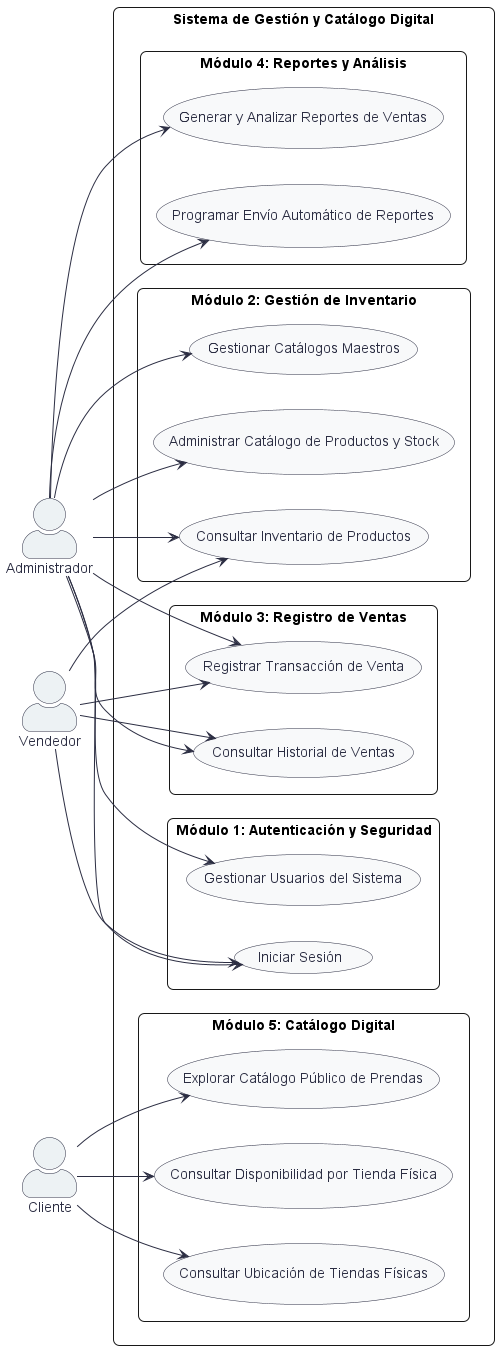
\includegraphics[width=0.92\textwidth]{cu_general_sistema.png}
\caption{Diagrama General de Casos de Uso del Sistema SYSELL Web (UML 2.5)}
\label{fig:cu_general}
\end{figure}

\subsection{Diagramas de Casos de Uso por Módulo Funcional}
A fin de asegurar máxima legibilidad y especificidad técnica, cada módulo funcional cuenta con su respectivo diagrama de interacción UML:

\begin{figure}[H]
\centering
\begin{minipage}{0.48\textwidth}
    \centering
    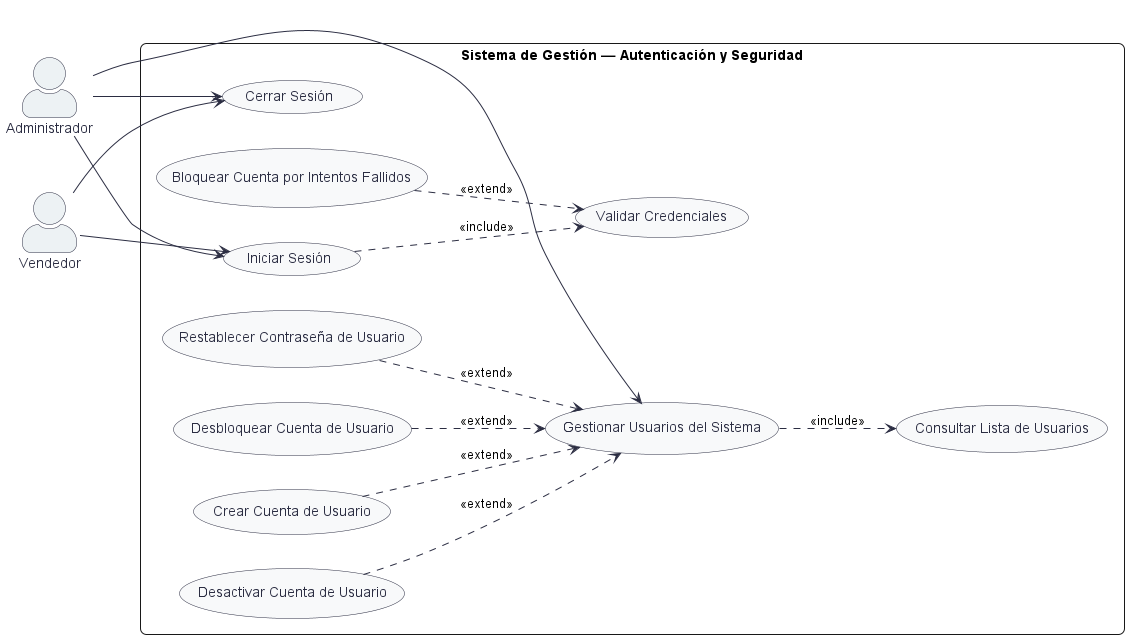
\includegraphics[width=\textwidth]{cu_modulo_1_autenticacion.png}
    \caption{Casos de Uso: Módulo 1 (Autenticación)}
    \label{fig:cu_m1}
\end{minipage}
\hfill
\begin{minipage}{0.48\textwidth}
    \centering
    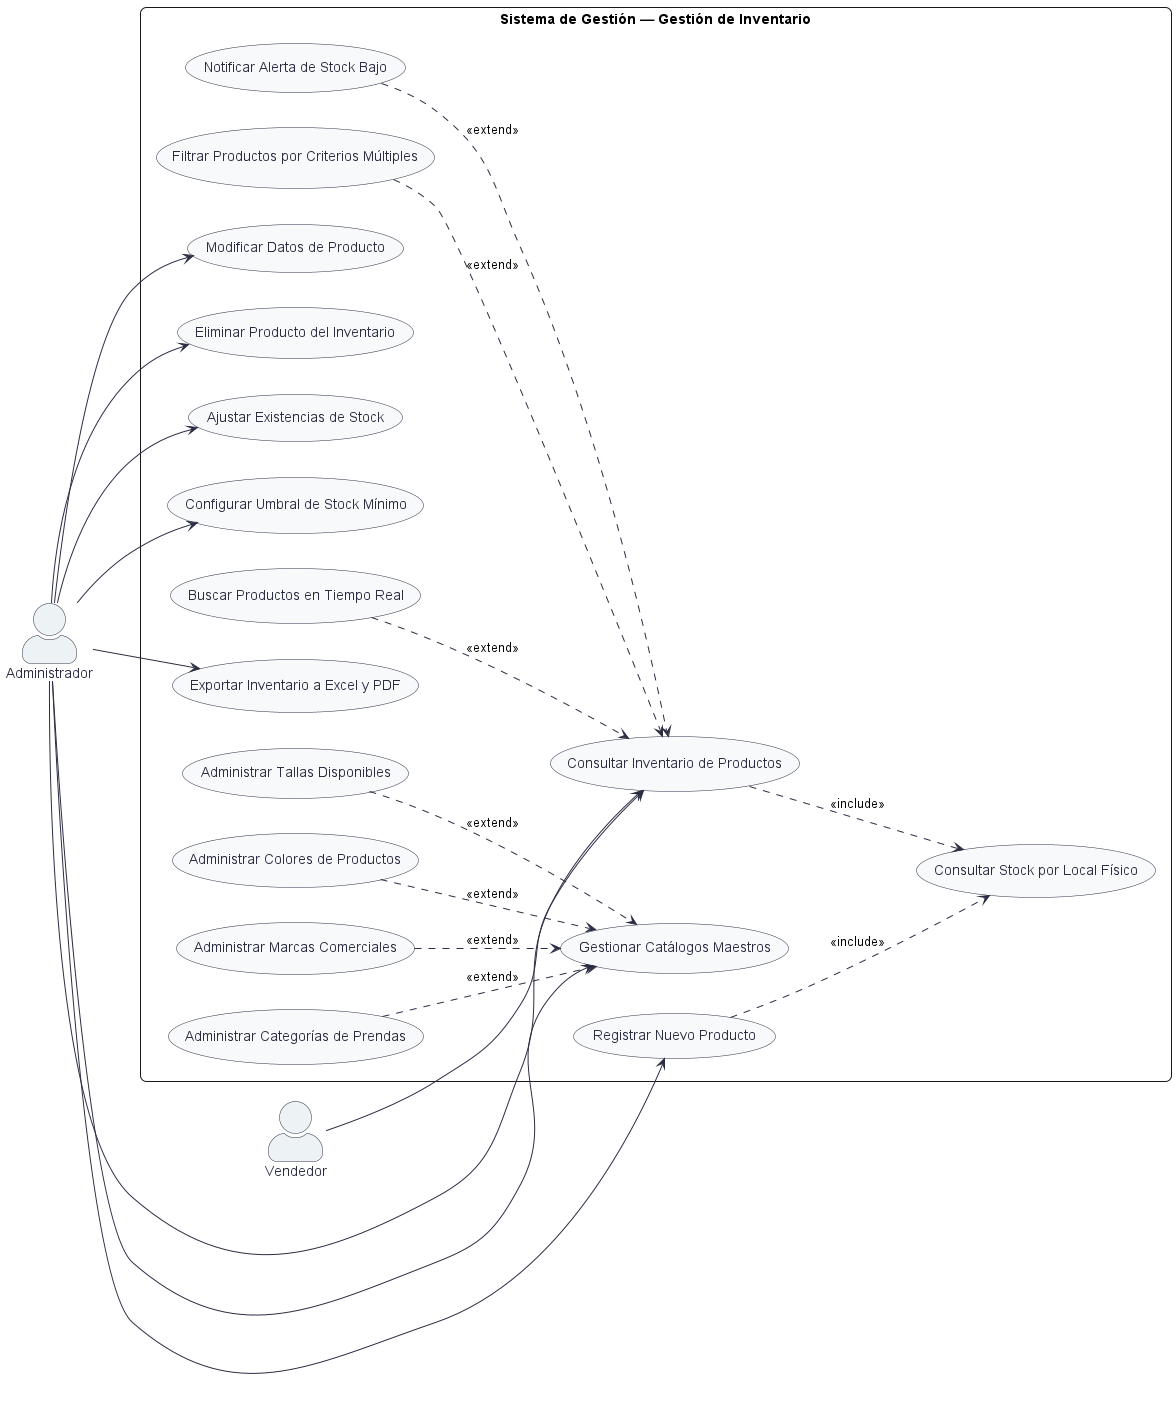
\includegraphics[width=\textwidth]{cu_modulo_2_inventario.png}
    \caption{Casos de Uso: Módulo 2 (Inventario)}
    \label{fig:cu_m2}
\end{minipage}
\end{figure}

\begin{figure}[H]
\centering
\begin{minipage}{0.48\textwidth}
    \centering
    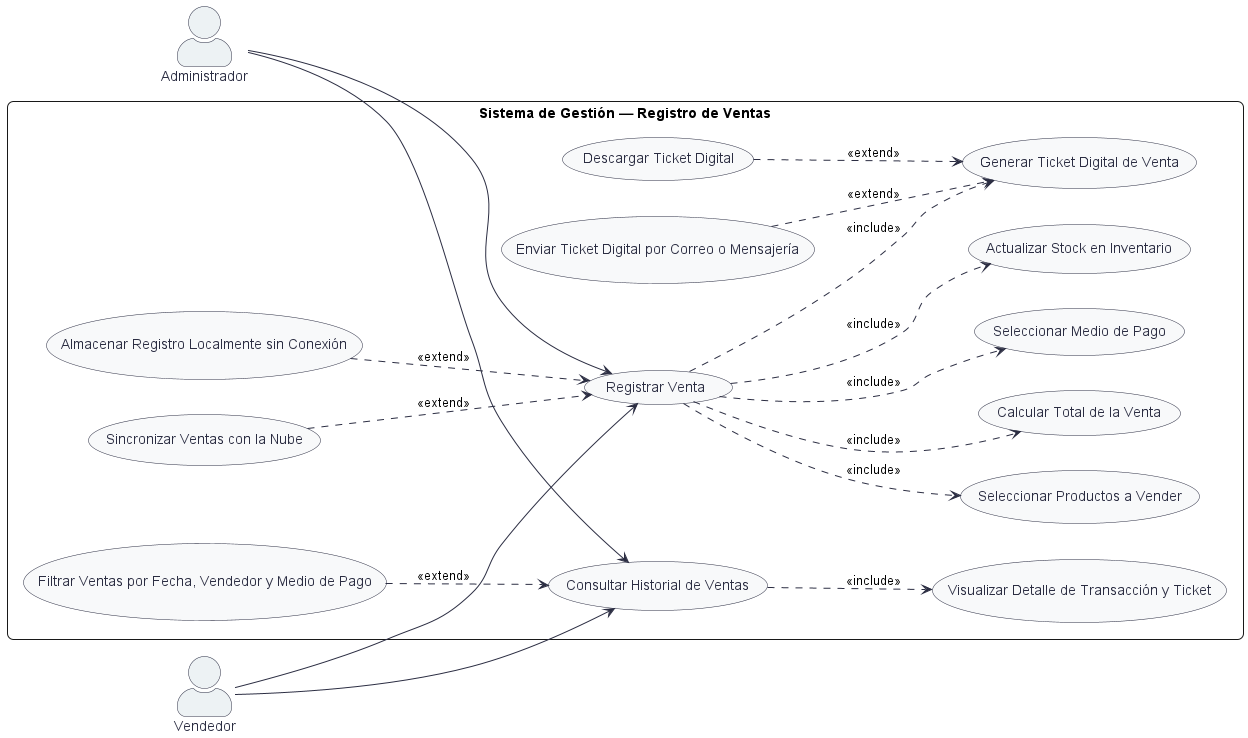
\includegraphics[width=\textwidth]{cu_modulo_3_ventas.png}
    \caption{Casos de Uso: Módulo 3 (Ventas POS)}
    \label{fig:cu_m3}
\end{minipage}
\hfill
\begin{minipage}{0.48\textwidth}
    \centering
    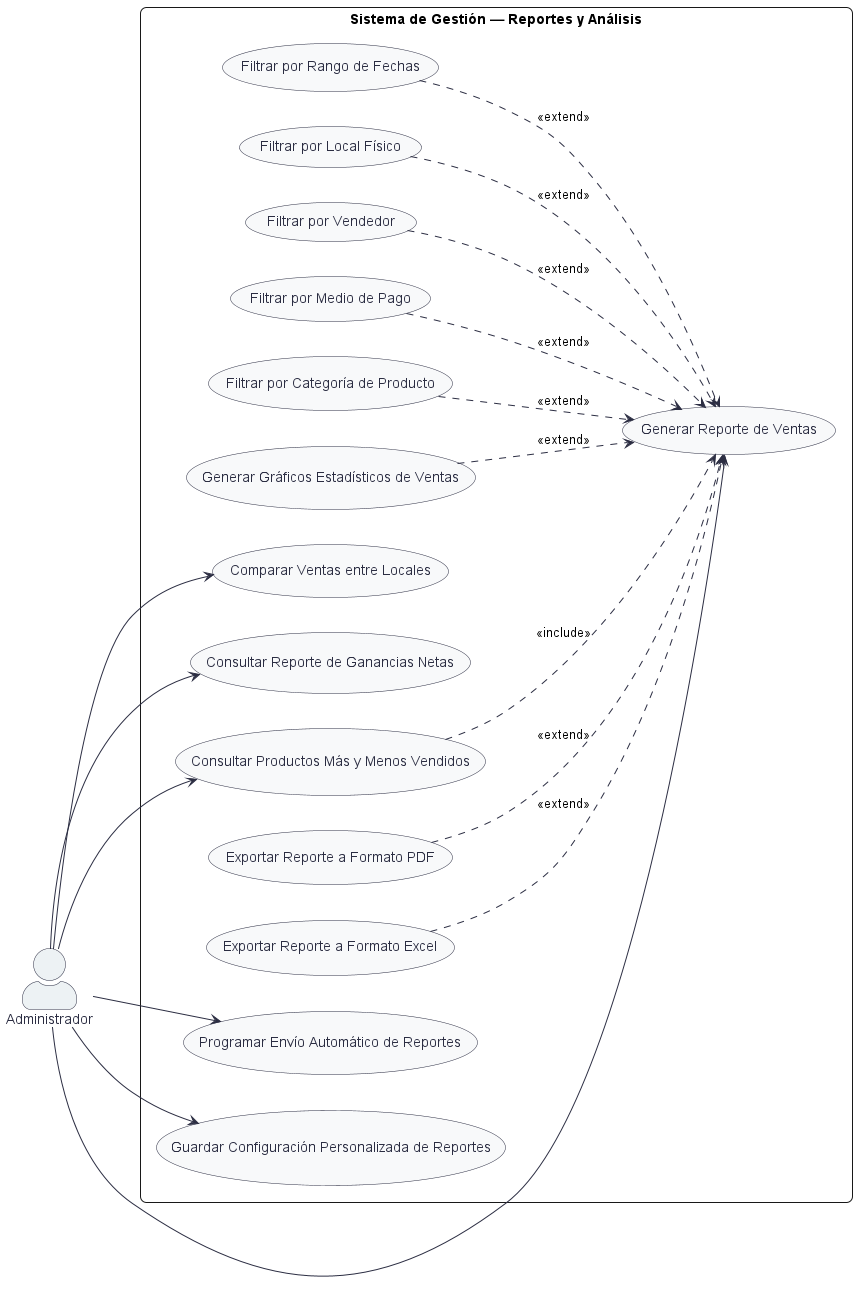
\includegraphics[width=\textwidth]{cu_modulo_4_reportes.png}
    \caption{Casos de Uso: Módulo 4 (Reportes)}
    \label{fig:cu_m4}
\end{minipage}
\end{figure}

\begin{figure}[H]
\centering
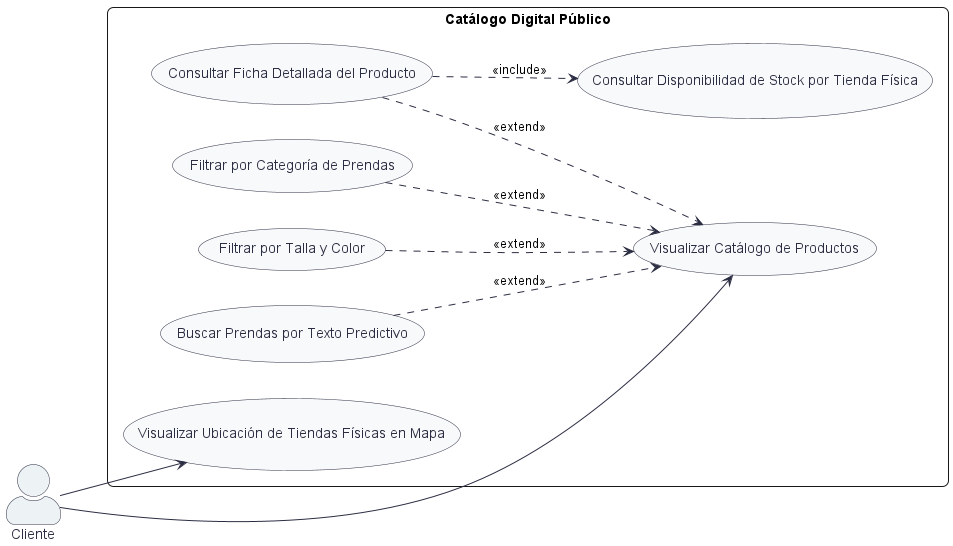
\includegraphics[width=0.6\textwidth]{cu_modulo_5_catalogo.png}
\caption{Casos de Uso: Módulo 5 (Catálogo Digital Público)}
\label{fig:cu_m5}
\end{figure}

\section{Diagramas de Flujo de Datos (DFD) Balanceados}
Para garantizar la consistencia en el tránsito de la información, se modeló el flujo de datos en tres niveles de abstracción balanceados conforme a la metodología de Yourdon/DeMarco:

\subsection{DFD Nivel 0: Diagrama de Contexto}
Delimita las fronteras del sistema informático e identifica los flujos esenciales con las entidades externas:

\begin{figure}[H]
\centering
\begin{tikzpicture}[
    scale=0.88, every node/.style={transform shape},
    entidad/.style={rectangle, draw=primaryblue!80!black, fill=primaryblue!10, rounded corners=3pt, thick, align=center, minimum width=3.2cm, minimum height=1.1cm, font=\small},
    proceso/.style={circle, draw=darkblue, fill=blue!15, line width=1.5pt, align=center, minimum size=3.6cm, font=\small\bfseries},
    dfdArrow/.style={thick, -{Stealth[length=2.2mm]}, primaryblue}
]
\node[proceso] (p0) at (0, 0) {0\\Sistema Web de\\Gestión SYSELL\\(Tienda Machi's)};

\node[entidad, draw=red!70!black, fill=red!10] (admin) at (0, 3.8) {\textbf{Administrador}\\\scriptsize (Propietario / Gerente)};
\node[entidad, draw=green!70!black, fill=green!10] (vendedor) at (-5.8, 0) {\textbf{Vendedor}\\\scriptsize (Caja / Mostrador)};
\node[entidad, draw=orange!70!black, fill=orange!10] (cliente) at (5.8, 0) {\textbf{Cliente Web}\\\scriptsize (Público Comprador)};

% Flujos Vendedor
\draw[dfdArrow] (vendedor.north east) -- node[midway, above=2pt, sloped, font=\scriptsize] {Credenciales, Ventas, Pagos} (p0.north west);
\draw[dfdArrow] (p0.south west) -- node[midway, below=2pt, sloped, font=\scriptsize] {Tickets, Vuelto, Stock local} (vendedor.south east);

% Flujos Administrador
\draw[dfdArrow] (admin.south west) -- node[midway, left=2pt, font=\scriptsize] {Parámetros, Catálogos, Ajustes} (p0.north west);
\draw[dfdArrow] (p0.north east) -- node[midway, right=2pt, font=\scriptsize] {Reportes, Alertas stock, Auditoría} (admin.south east);

% Flujos Cliente Web
\draw[dfdArrow] (cliente.north west) -- node[midway, above=2pt, sloped, font=\scriptsize] {Filtros y búsquedas web} (p0.north east);
\draw[dfdArrow] (p0.south east) -- node[midway, below=2pt, sloped, font=\scriptsize] {Catálogo HD, Disponibilidad tienda} (cliente.south west);

\end{tikzpicture}
\caption{Diagrama de Flujo de Datos: Nivel 0 (Diagrama de Contexto)}
\label{fig:dfd_nivel_0}
\end{figure}

\subsection{DFD Nivel 1: Procesos Principales del Sistema}
Descompone el sistema en cinco procesos macro interconectados con los cinco almacenes de datos normalizados:

\begin{figure}[H]
\centering
\begin{tikzpicture}[
    scale=0.82, every node/.style={transform shape},
    proceso/.style={circle, draw=primaryblue!80!black, fill=primaryblue!10, thick, align=center, minimum size=2.2cm, font=\scriptsize\bfseries},
    almacen/.style={rectangle, draw=purple!80!black, fill=purple!10, rounded corners=2pt, thick, align=center, minimum width=2.8cm, minimum height=0.7cm, font=\scriptsize},
    entidad/.style={rectangle, draw=darkblue, fill=blue!10, rounded corners=2pt, thick, align=center, minimum width=2.6cm, minimum height=0.8cm, font=\scriptsize\bfseries},
    flow/.style={thick, -{Stealth[length=2mm]}, primaryblue}
]
% Entidades
\node[entidad, fill=red!10, draw=red!70!black] (eAdmin) at (-5.5, 3.5) {Administrador};
\node[entidad, fill=green!10, draw=green!70!black] (eVend) at (0, 3.5) {Vendedor};
\node[entidad, fill=orange!10, draw=orange!70!black] (eCli) at (5.5, 3.5) {Cliente Web};

% Procesos
\node[proceso] (p1) at (-4.5, 1.2) {1.0\\Autenticar\\y Usuarios};
\node[proceso] (p2) at (-1.5, 1.2) {2.0\\Gestionar\\Inventario};
\node[proceso] (p3) at (1.5, 1.2) {3.0\\Procesar\\Ventas POS};
\node[proceso] (p4) at (-3, -1.8) {4.0\\Generar\\Reportes};
\node[proceso] (p5) at (4.5, 1.2) {5.0\\Catálogo\\Digital Web};

% Almacenes
\node[almacen] (d1) at (-4.5, -0.2) {D1: Usuarios y Roles};
\node[almacen] (d2) at (-0.5, -0.2) {D2: Catálogos Maestros};
\node[almacen] (d3) at (2.8, -0.2) {D3: Inventario y Kardex};
\node[almacen] (d4) at (0, -1.8) {D4: Ventas y Tickets};
\node[almacen] (d5) at (3.5, -1.8) {D5: Auditoría};

% Conexiones
\draw[flow] (eAdmin) -- (p1);
\draw[flow] (eVend) -- (p1);
\draw[flow] (p1) -- (d1);
\draw[flow] (eAdmin) -- (p2);
\draw[flow] (p2) -- (d2);
\draw[flow] (p2) -- (d3);
\draw[flow] (eVend) -- (p3);
\draw[flow] (p3) -- (d3);
\draw[flow] (p3) -- (d4);
\draw[flow] (p3) -- (d5);
\draw[flow] (eAdmin) -- (p4);
\draw[flow] (d4) -- (p4);
\draw[flow] (eCli) -- (p5);
\draw[flow] (d3) -- (p5);

\end{tikzpicture}
\caption{Diagrama de Flujo de Datos: Nivel 1 (Procesos Principales y Almacenes D1--D5)}
\label{fig:dfd_nivel_1}
\end{figure}

\subsection{DFD Nivel 2: Descomposición del Proceso de Ventas (P 3.0)}
Desglosa la lógica transaccional de caja en cinco subprocesos atómicos:

\begin{figure}[H]
\centering
\begin{tikzpicture}[
    scale=0.85, every node/.style={transform shape},
    subproc/.style={circle, draw=primaryblue!80!black, fill=primaryblue!10, thick, align=center, minimum size=1.9cm, font=\scriptsize\bfseries},
    store/.style={rectangle, draw=purple!80!black, fill=purple!10, rounded corners=2pt, thick, align=center, minimum width=2.6cm, minimum height=0.6cm, font=\scriptsize},
    flow/.style={thick, -{Stealth[length=2mm]}, primaryblue}
]
\node[subproc] (p31) at (0, 0) {3.1\\Validar Stock\\y Prenda};
\node[subproc] (p32) at (3.0, 0) {3.2\\Calcular\\Totales};
\node[subproc] (p33) at (6.0, 0) {3.3\\Registrar\\Cobro};
\node[subproc] (p34) at (9.0, 0) {3.4\\Actualizar\\Inventario};
\node[subproc] (p35) at (12.0, 0) {3.5\\Emitir\\Ticket};

\node[store] (d3) at (0, -1.8) {D3: Inventario};
\node[store] (d4) at (12.0, -1.8) {D4: Ventas};
\node[store] (d5) at (9.0, -1.8) {D5: Kardex};

\draw[flow] (p31) -- (p32);
\draw[flow] (p32) -- (p33);
\draw[flow] (p33) -- (p34);
\draw[flow] (p34) -- (p35);

\draw[flow] (d3) -- (p31);
\draw[flow] (p34) -- (d3);
\draw[flow] (p34) -- (d5);
\draw[flow] (p35) -- (d4);

\end{tikzpicture}
\caption{Diagrama de Flujo de Datos: Nivel 2 (Descomposición del Proceso de Ventas 3.0)}
\label{fig:dfd_nivel_2}
\end{figure}

\section{Diccionario de Almacenes de Datos Normalizados (D1 a D5)}
\begin{table}[H]
\centering
\small
\begin{tabularx}{\textwidth}{>{\ttfamily\centering}p{1.2cm} >{\raggedright\bfseries}p{3.8cm} >{\ttfamily\small\raggedright}p{4cm} Y}
\toprule
\textbf{Almacén} & \textbf{Nombre del Almacén} & \textbf{Tablas Relacionales Asociadas} & \textbf{Contenido y Finalidad} \\
\midrule
D1 & Usuarios y Roles & usuarios, locales & Cuentas, credenciales Bcrypt, roles RBAC y asignación física de locales. \\
\addlinespace
D2 & Catálogos Maestros & categorias, marcas, tallas, colores & Listas cerradas inmutables para selección de atributos de prendas (RF-74). \\
\addlinespace
D3 & Inventario y Kardex & productos, variantes\_producto, inventario, ajustes\_inventario & Existencias por tienda, SKUs normalizados, alertas de stock y auditoría de Kardex. \\
\addlinespace
D4 & Ventas y Comprobantes & ventas, detalle\_ventas, pagos\_venta, metodos\_pago & Encabezados, desglose de prendas vendidas, importes, medios mixtos y tickets. \\
\addlinespace
D5 & Bitácora y Auditoría & auditoria, reportes\_configuracion & Registro inmutable de eventos críticos (crear, anular, resetear) con detalle JSON. \\
\bottomrule
\end{tabularx}
\caption{Mapeo formal de almacenes de datos DFD a tablas de la base de datos MySQL}
\label{tab:almacenes_dfd}
\end{table}

\chapter{Diseño Dinámico e Interacción Técnica (PlantUML)}

\section{Estándar de Modelado Dinámico en PlantUML}
A diferencia de los diagramas conceptuales abstractos, los diagramas de secuencia de \textbf{SYSELL Web v2.0} fueron codificados en \textbf{PlantUML} bajo la directiva \texttt{skinparam style strictuml}. Cada diagrama modela con exactitud los mensajes síncronos y asíncronos que atraviesan las cuatro capas de la arquitectura del software:
\begin{enumerate}
    \item \textbf{Capa de Presentación (UI / SPA):} Cliente web interactivo en React 18 / TypeScript.
    \item \textbf{Capa de Controladores API:} Endpoints RESTful en Laravel que aplican validaciones de formulario, sanitización y middlewares de autorización.
    \item \textbf{Capa de Aplicación (Application Service):} Handlers de Commands y Queries que orquestan las reglas de negocio desacopladas.
    \item \textbf{Capa de Dominio y Persistencia:} Entidades de negocio y Repositorios que interactúan con MySQL 8.0 bajo transacciones ACID.
\end{enumerate}

\section{Catálogo de los 8 Diagramas de Secuencia Técnicos}
Se diseñaron 8 diagramas de secuencia que cubren la totalidad de los flujos críticos del sistema:

\begin{table}[H]
\centering
\small
\begin{tabularx}{\textwidth}{>{\ttfamily\centering}p{1.4cm} >{\raggedright\bfseries}p{4cm} >{\ttfamily\centering}p{1.8cm} Y}
\toprule
\textbf{Código} & \textbf{Diagrama de Secuencia} & \textbf{Caso de Uso} & \textbf{Lógica Técnica Modelada} \\
\midrule
DS-01 & Autenticación JWT y Bloqueo & CU-01 & Verificación Bcrypt, generación de token y bloqueo automático al 3er fallo consecutivo. \\
\addlinespace
DS-02 & Registro de Prendas y Catálogos & CU-05, CU-07 & Validación de atributos en catálogos cerrados, cálculo de SKU único y persistencia. \\
\addlinespace
DS-03 & Transacción de Venta POS & CU-08, CU-09 & Validación de stock, liquidación con pagos mixtos, descuento atómico y ticket digital. \\
\addlinespace
DS-04 & Ajuste de Stock en Kardex & CU-06 & Asiento manual por el Administrador con justificación obligatoria y recálculo de saldo. \\
\addlinespace
DS-05 & Reporte y Exportación de Ventas & CU-13, CU-14 & Consultas agregadas con filtros multicriterio y compilación en PDF/Excel. \\
\addlinespace
DS-06 & Gestión y Desbloqueo de Usuarios & CU-02 & CRUD de colaboradores, cambio de local, reseteo de clave y reinicio de intentos a 0. \\
\addlinespace
DS-07 & Catálogo Digital Web Público & CU-15 & Consulta pública sin autenticación, filtros AND y stock referencial por tienda física. \\
\addlinespace
DS-08 & Anulación de Venta Comercial & CU-12 & Validación de clave de Admin, cambio de estado y restitución atómica de existencias. \\
\bottomrule
\end{tabularx}
\caption{Suite de Diagramas de Secuencia Técnicos formalizados en SYSELL Web}
\label{tab:diagramas_secuencia}
\end{table}

\section{Análisis de Flujos Transaccionales Críticos con Evidencia Gráfica}

\subsection{Autenticación y Bloqueo Preventivo (DS-01)}
El flujo modela la recepción del payload JSON con credenciales en \texttt{/api/auth/login}. El servicio recupera el usuario por su \texttt{username}; si la cuenta no está bloqueada ni inactiva, compara la clave recibida mediante \texttt{password\_verify()} con el hash almacenado. Si la verificación falla:
\begin{lstlisting}[language=SQL]
UPDATE usuarios 
SET intentos_fallidos = intentos_fallidos + 1,
    bloqueado = CASE WHEN intentos_fallidos + 1 >= 3 THEN 1 ELSE 0 END
WHERE id = ?;
\end{lstlisting}
Si el contador alcanza 3, el estado pasa de inmediato a \texttt{bloqueado = 1}, denegando futuras peticiones y registrando el evento en la bitácora de auditoría.

\begin{figure}[H]
\centering
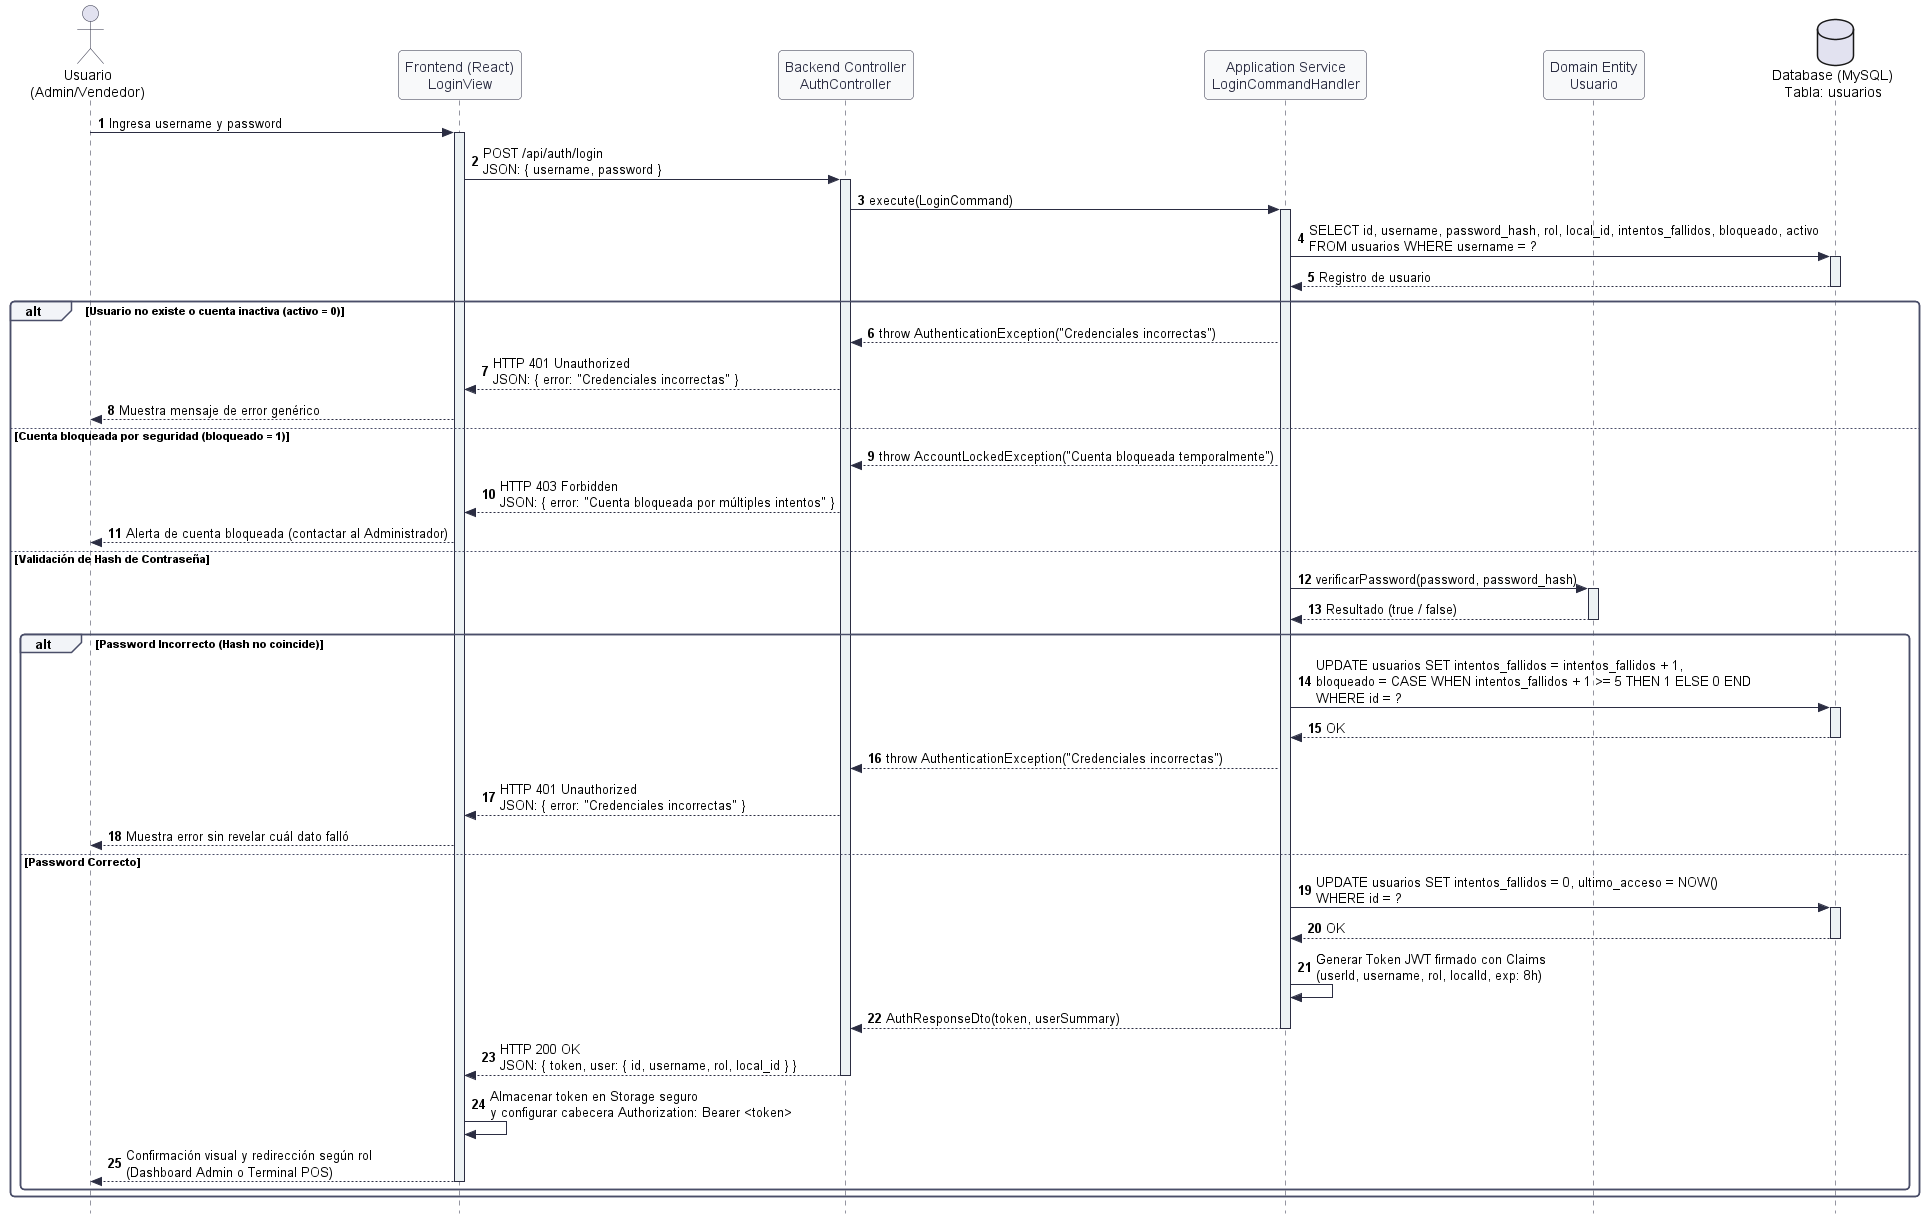
\includegraphics[width=0.92\textwidth]{ds_01_autenticacion_jwt.png}
\caption{Diagrama de Secuencia DS-01: Autenticación JWT y Bloqueo al 3er Intento}
\label{fig:ds_01}
\end{figure}

\subsection{Registro de Prendas y Desglose de Variantes (DS-02)}
El administrador registra una prenda base vinculándola a catálogos cerrados. El sistema genera de forma cartesiana las variantes de talla y color asignando los códigos SKU normalizados:

\begin{figure}[H]
\centering
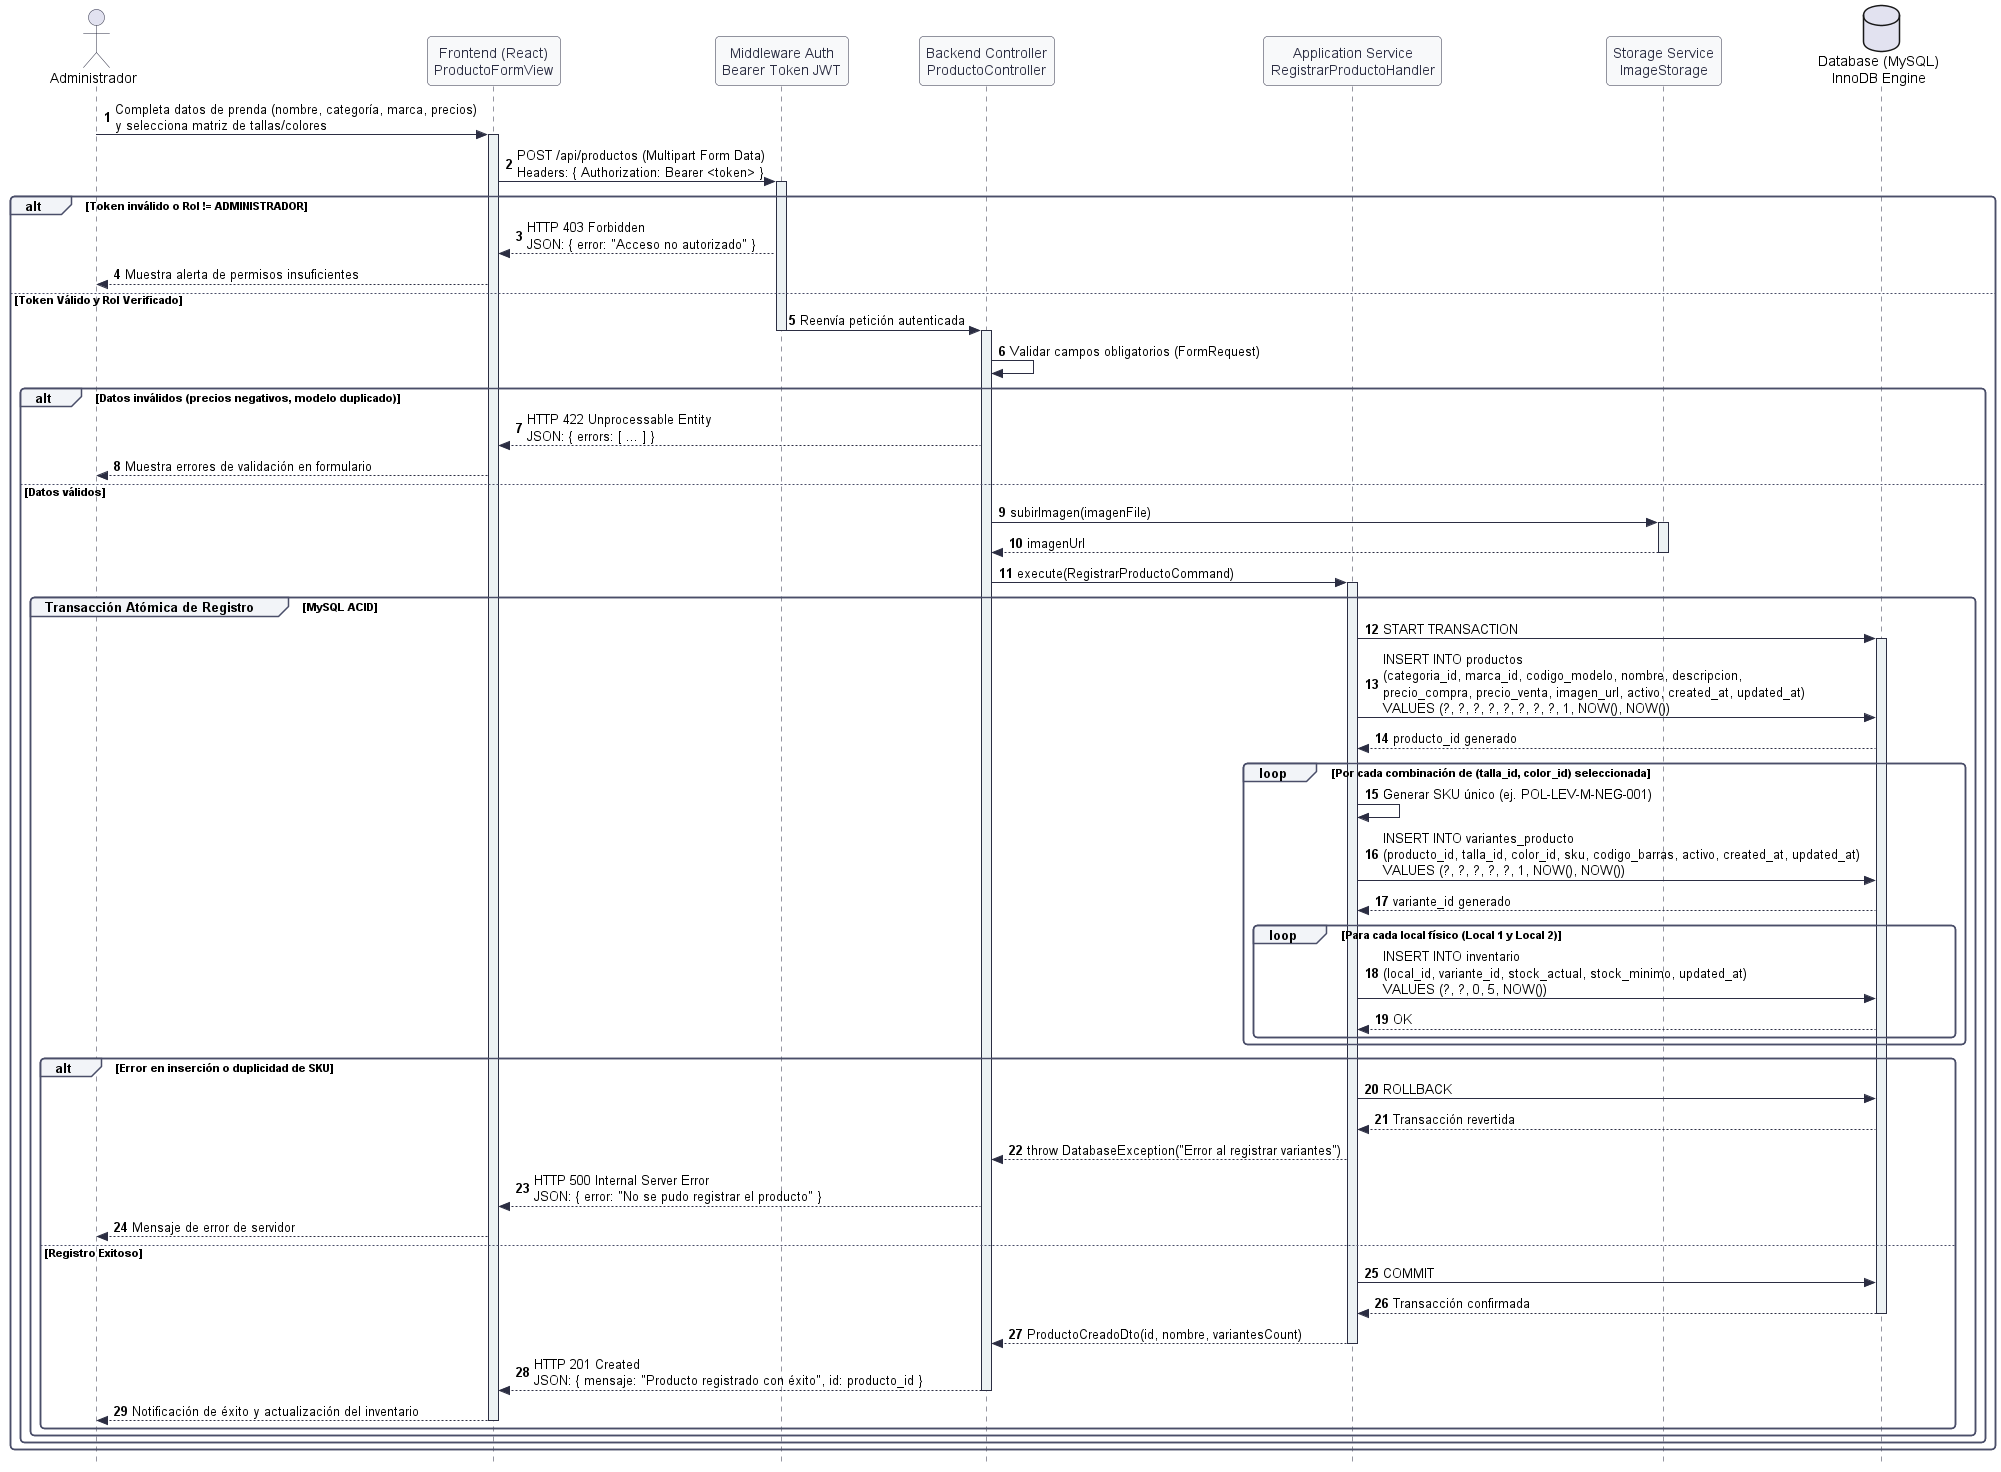
\includegraphics[width=0.92\textwidth]{ds_02_registro_producto_variantes.png}
\caption{Diagrama de Secuencia DS-02: Registro de Prenda Base y Variantes por SKU}
\label{fig:ds_02}
\end{figure}

\subsection{Transacción Atómica de Venta POS (DS-03)}
Para evitar inconsistencias en el inventario ante concurrencia o caídas de red, el proceso de confirmación de venta se ejecuta dentro de una transacción ACID (\textit{Database Transaction}):
\begin{enumerate}
    \item Inicio de transacción (\texttt{START TRANSACTION}).
    \item Inserción del encabezado en \texttt{ventas} con numeración correlativa única (\texttt{numero\_ticket}).
    \item Inserción de las líneas en \texttt{detalle\_ventas}.
    \item Descuento de stock en la tabla \texttt{inventario} para el local emisor:
    \begin{lstlisting}[language=SQL]
    UPDATE inventario 
    SET stock_actual = stock_actual - ? 
    WHERE local_id = ? AND variante_id = ? AND stock_actual >= ?;
    \end{lstlisting}
    \item Inserción de los medios de pago aplicados en \texttt{pagos\_venta}.
    \item Confirmación definitiva (\texttt{COMMIT}). En caso de cualquier falla de validación o stock insuficiente, se aborta la operación completa (\texttt{ROLLBACK}).
\end{enumerate}

\begin{figure}[H]
\centering
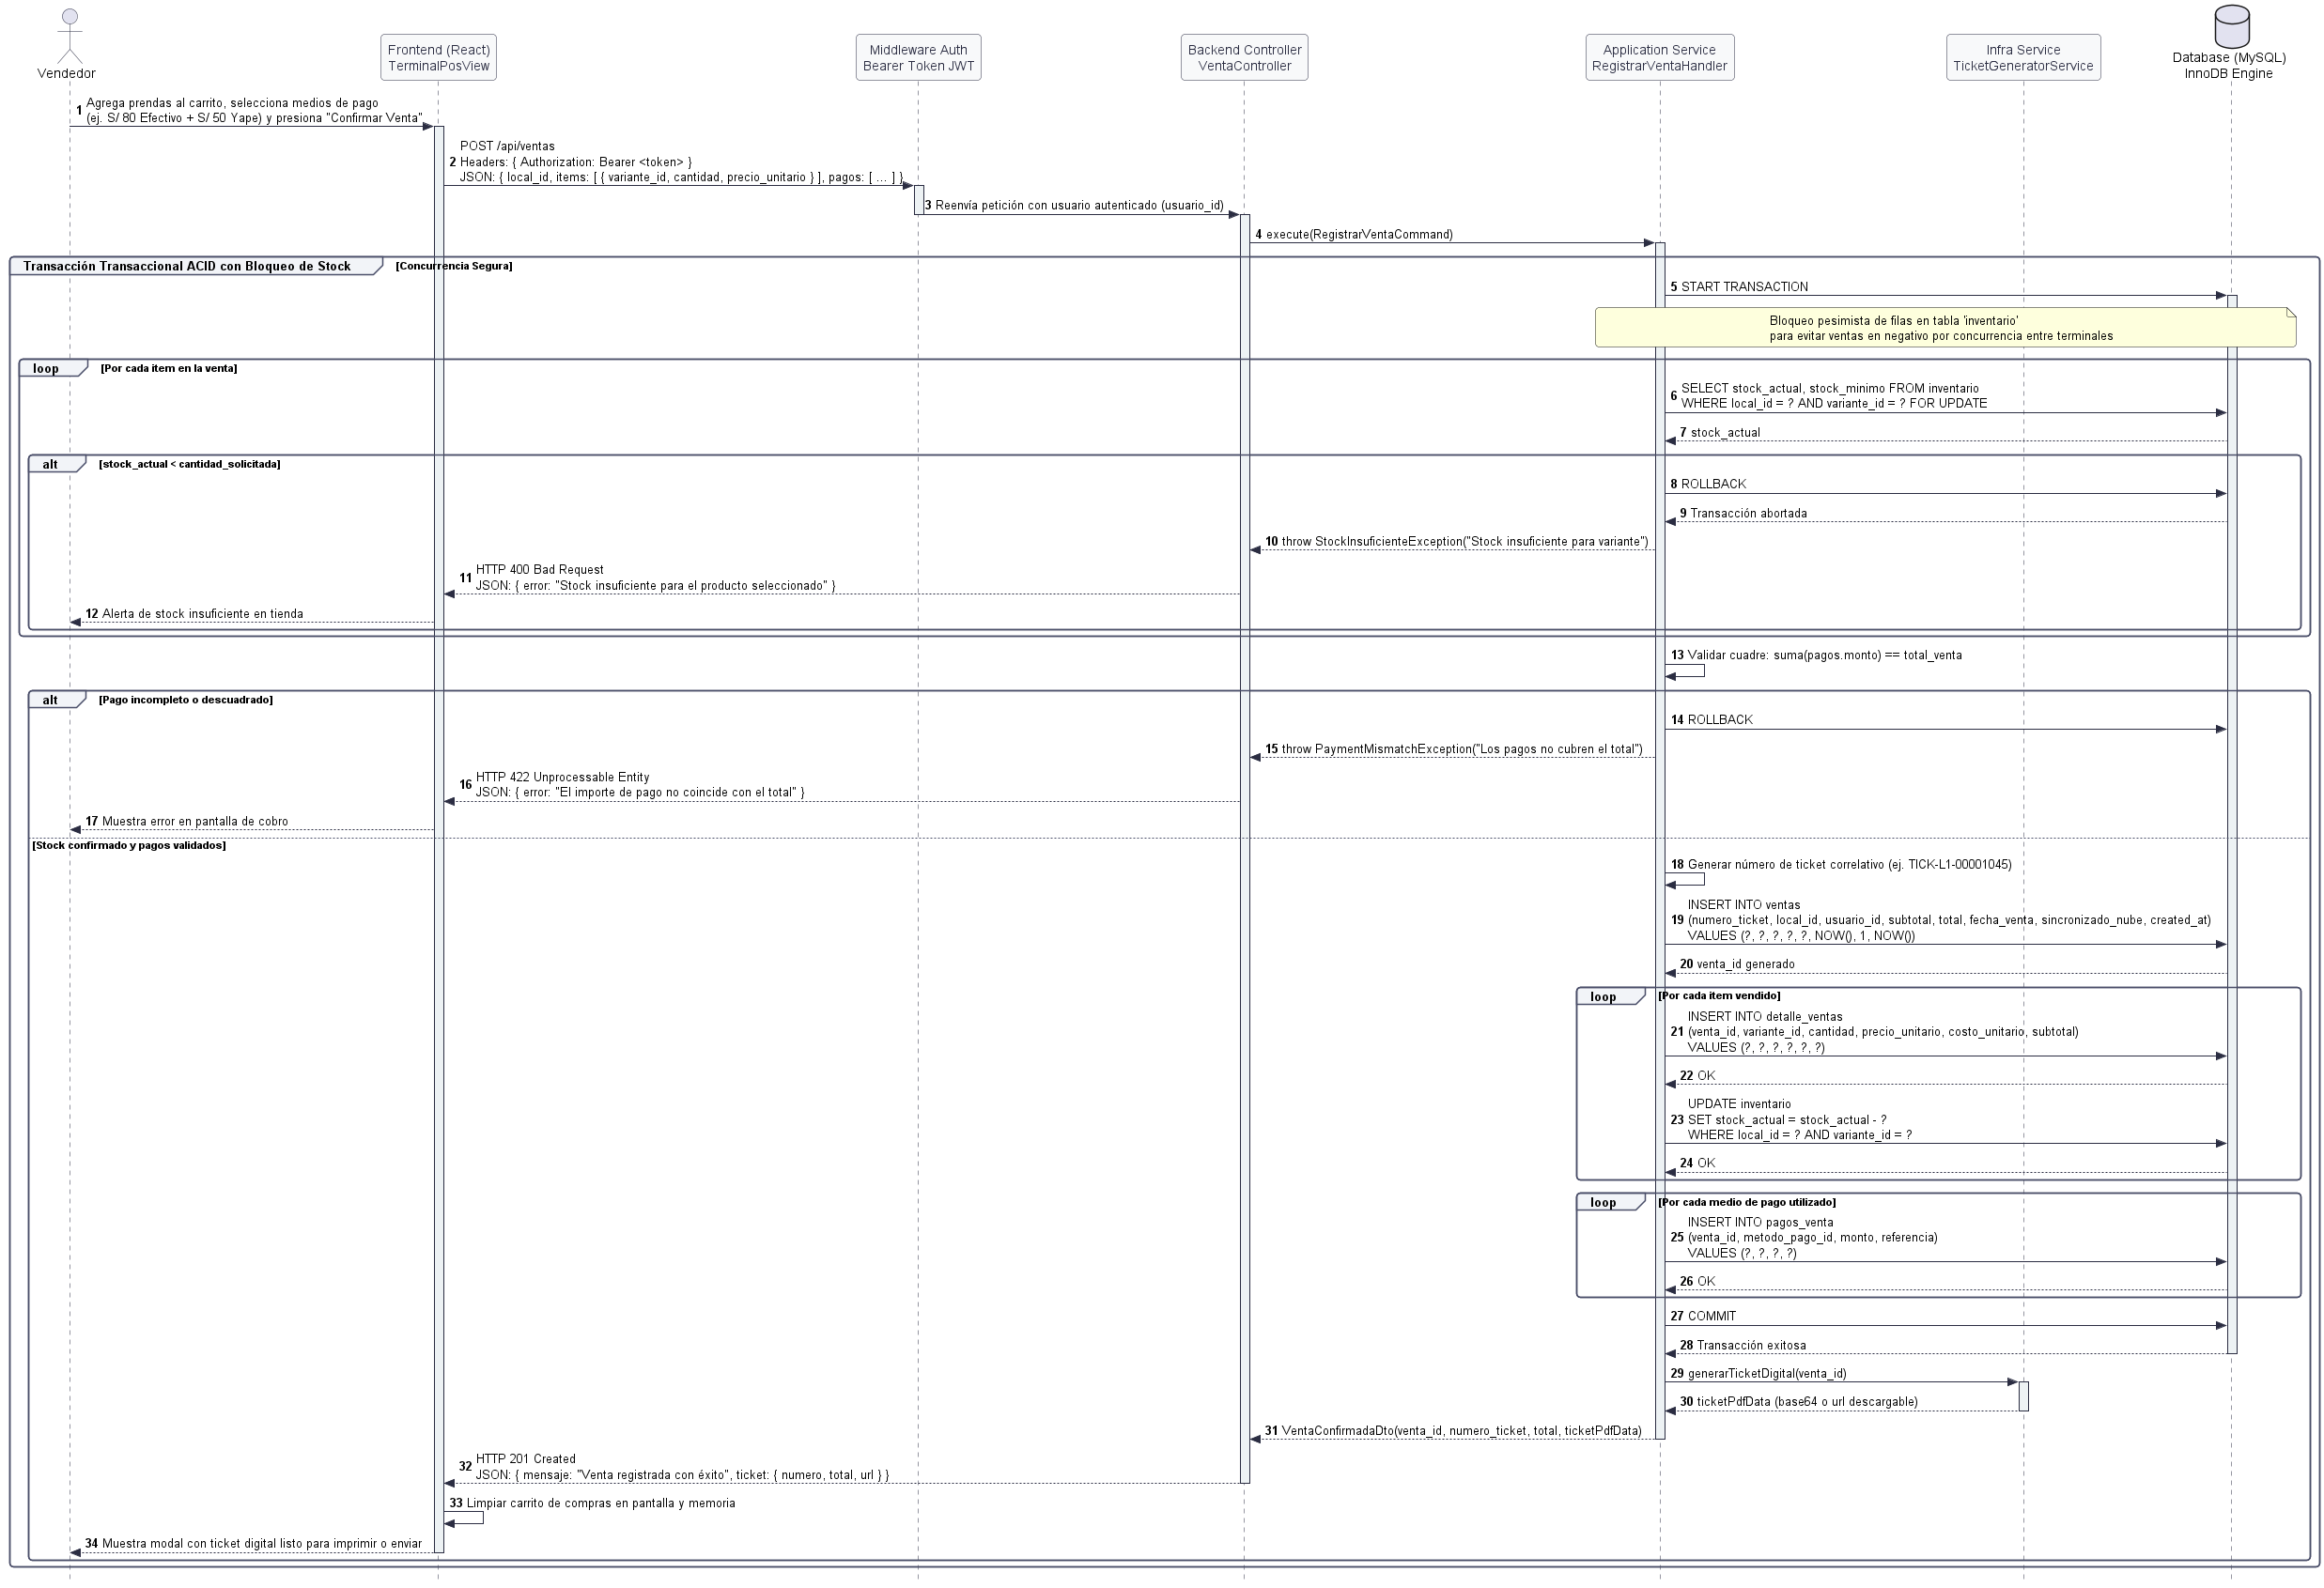
\includegraphics[width=0.92\textwidth]{ds_03_transaccion_venta_pos.png}
\caption{Diagrama de Secuencia DS-03: Transacción Atómica de Venta en Terminal POS}
\label{fig:ds_03}
\end{figure}

\subsection{Ajuste Manual de Existencias en Kardex (DS-04)}
Cualquier modificación manual del inventario físico requiere autorización del administrador, motivo explícito y registro de saldo previo y posterior:

\begin{figure}[H]
\centering
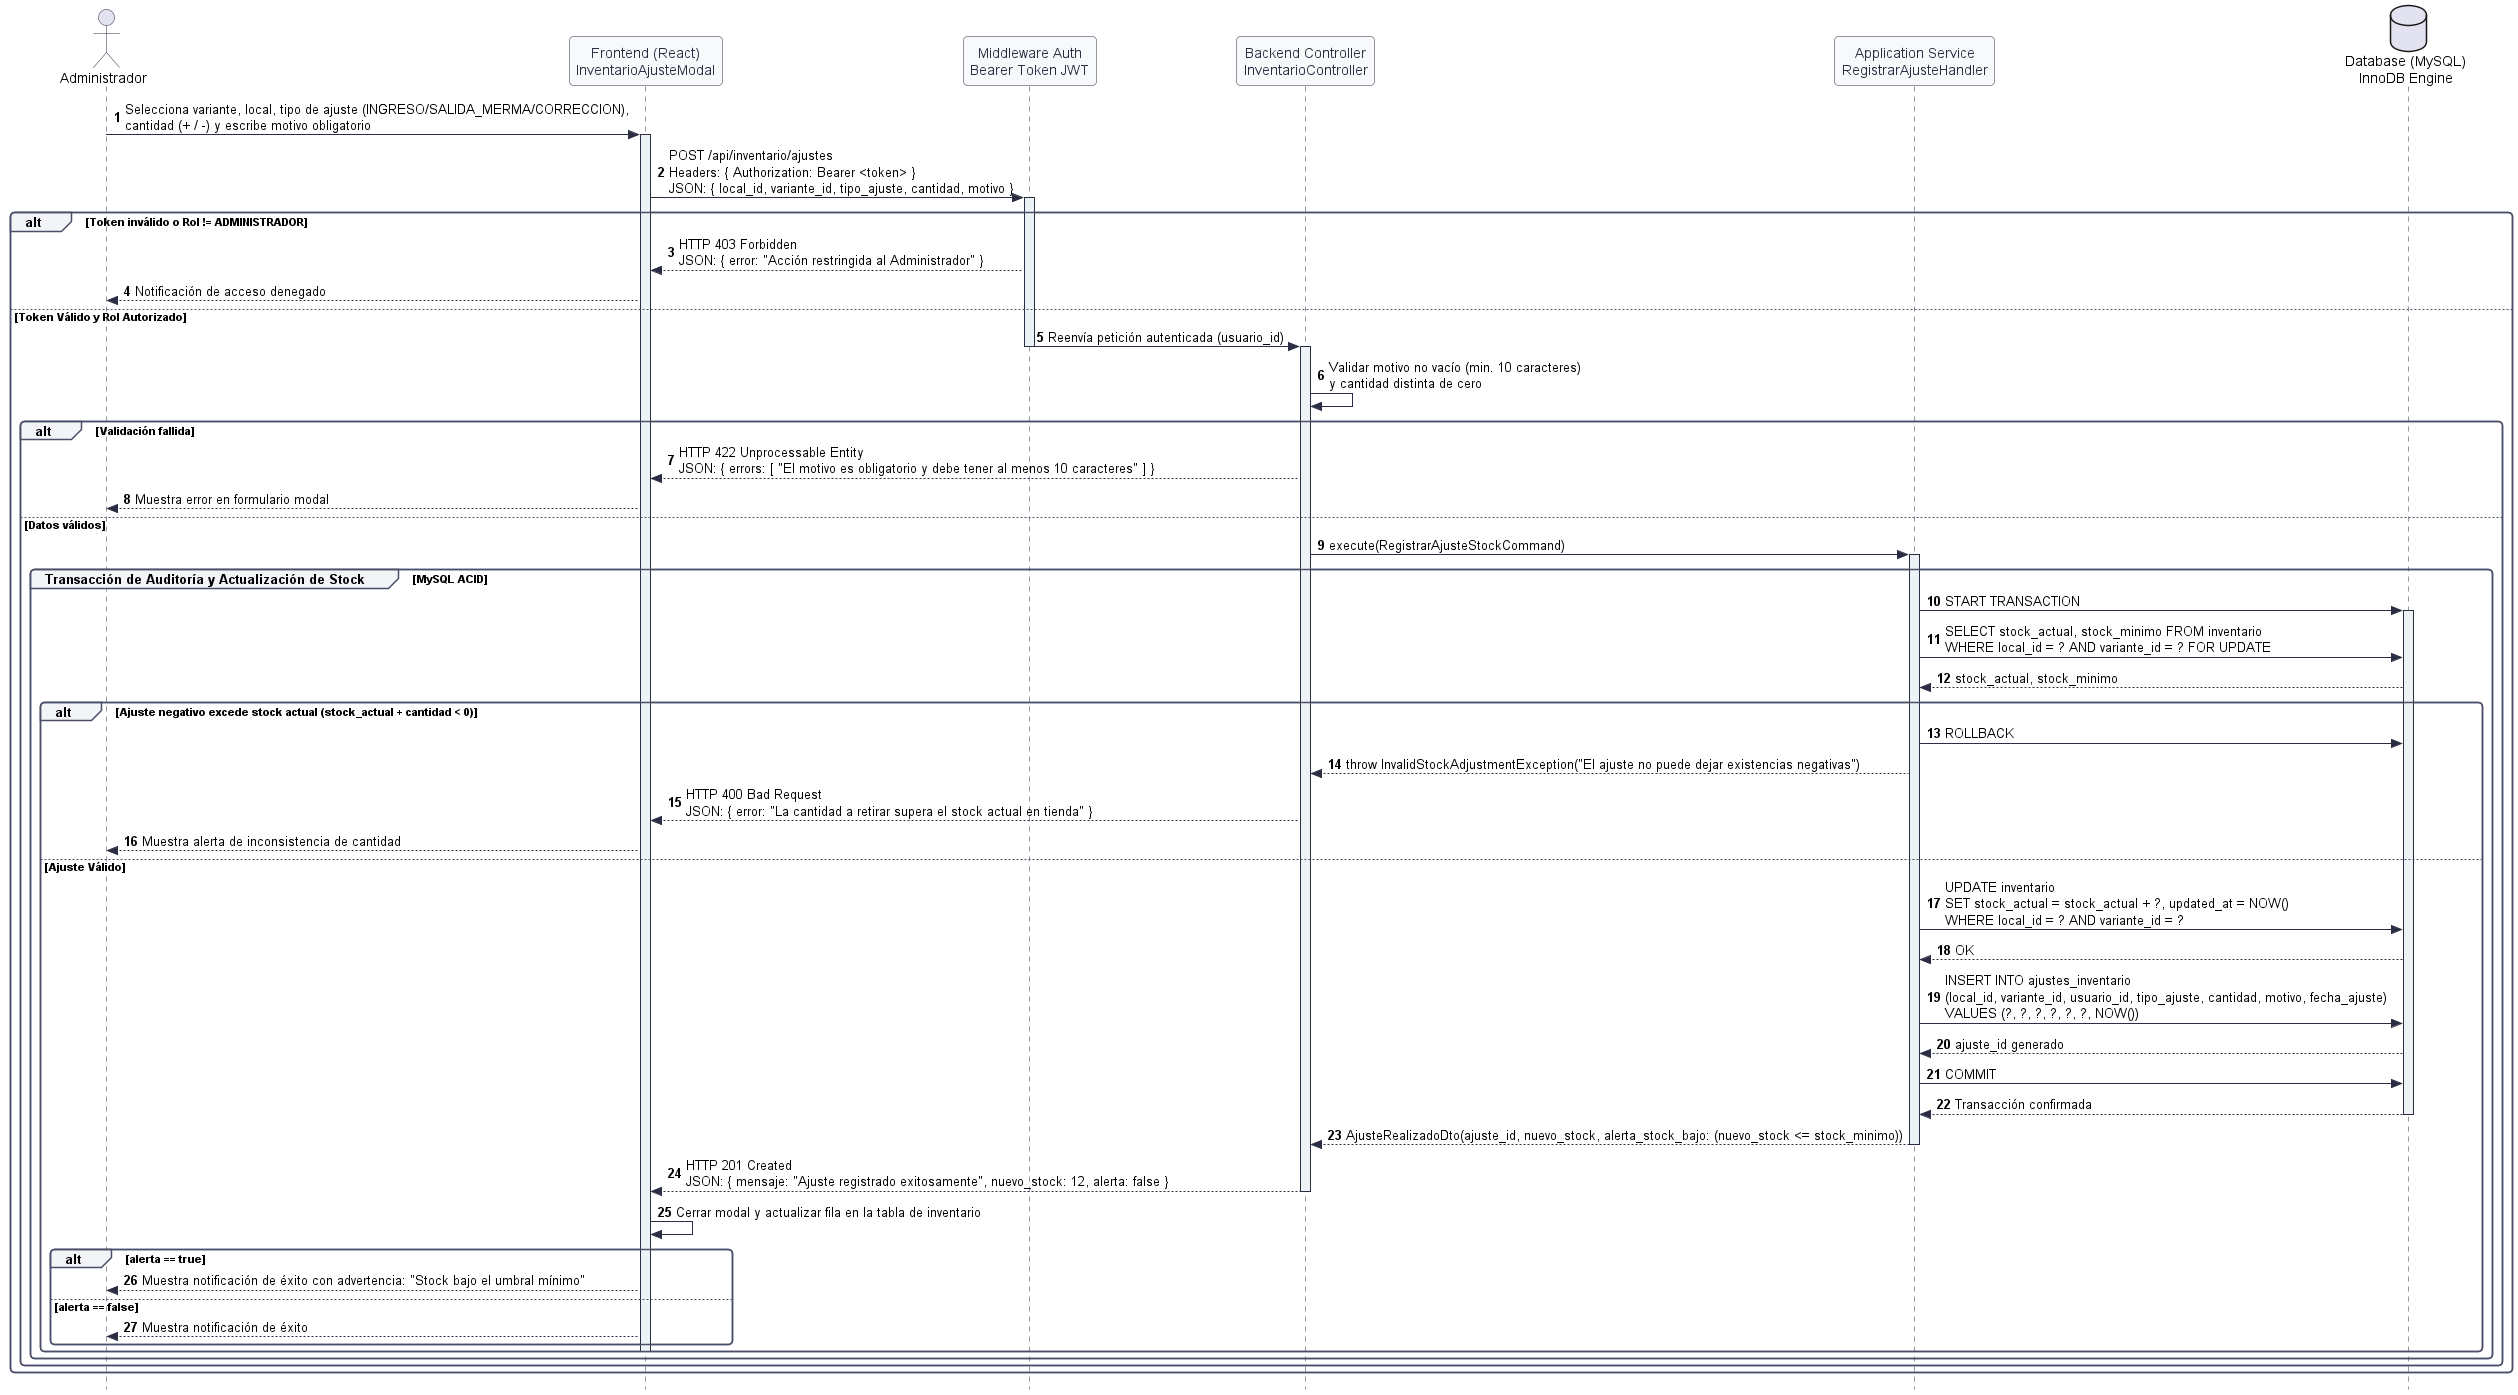
\includegraphics[width=0.92\textwidth]{ds_04_ajuste_inventario_kardex.png}
\caption{Diagrama de Secuencia DS-04: Ajuste de Inventario Físico y Movimiento de Kardex}
\label{fig:ds_04}
\end{figure}

\subsection{Generación y Exportación de Reportes Gerenciales (DS-05)}
Las consultas analíticas leen vistas optimizadas agregando ventas por sucursal, vendedor y rotación sin bloquear las tablas de caja:

\begin{figure}[H]
\centering
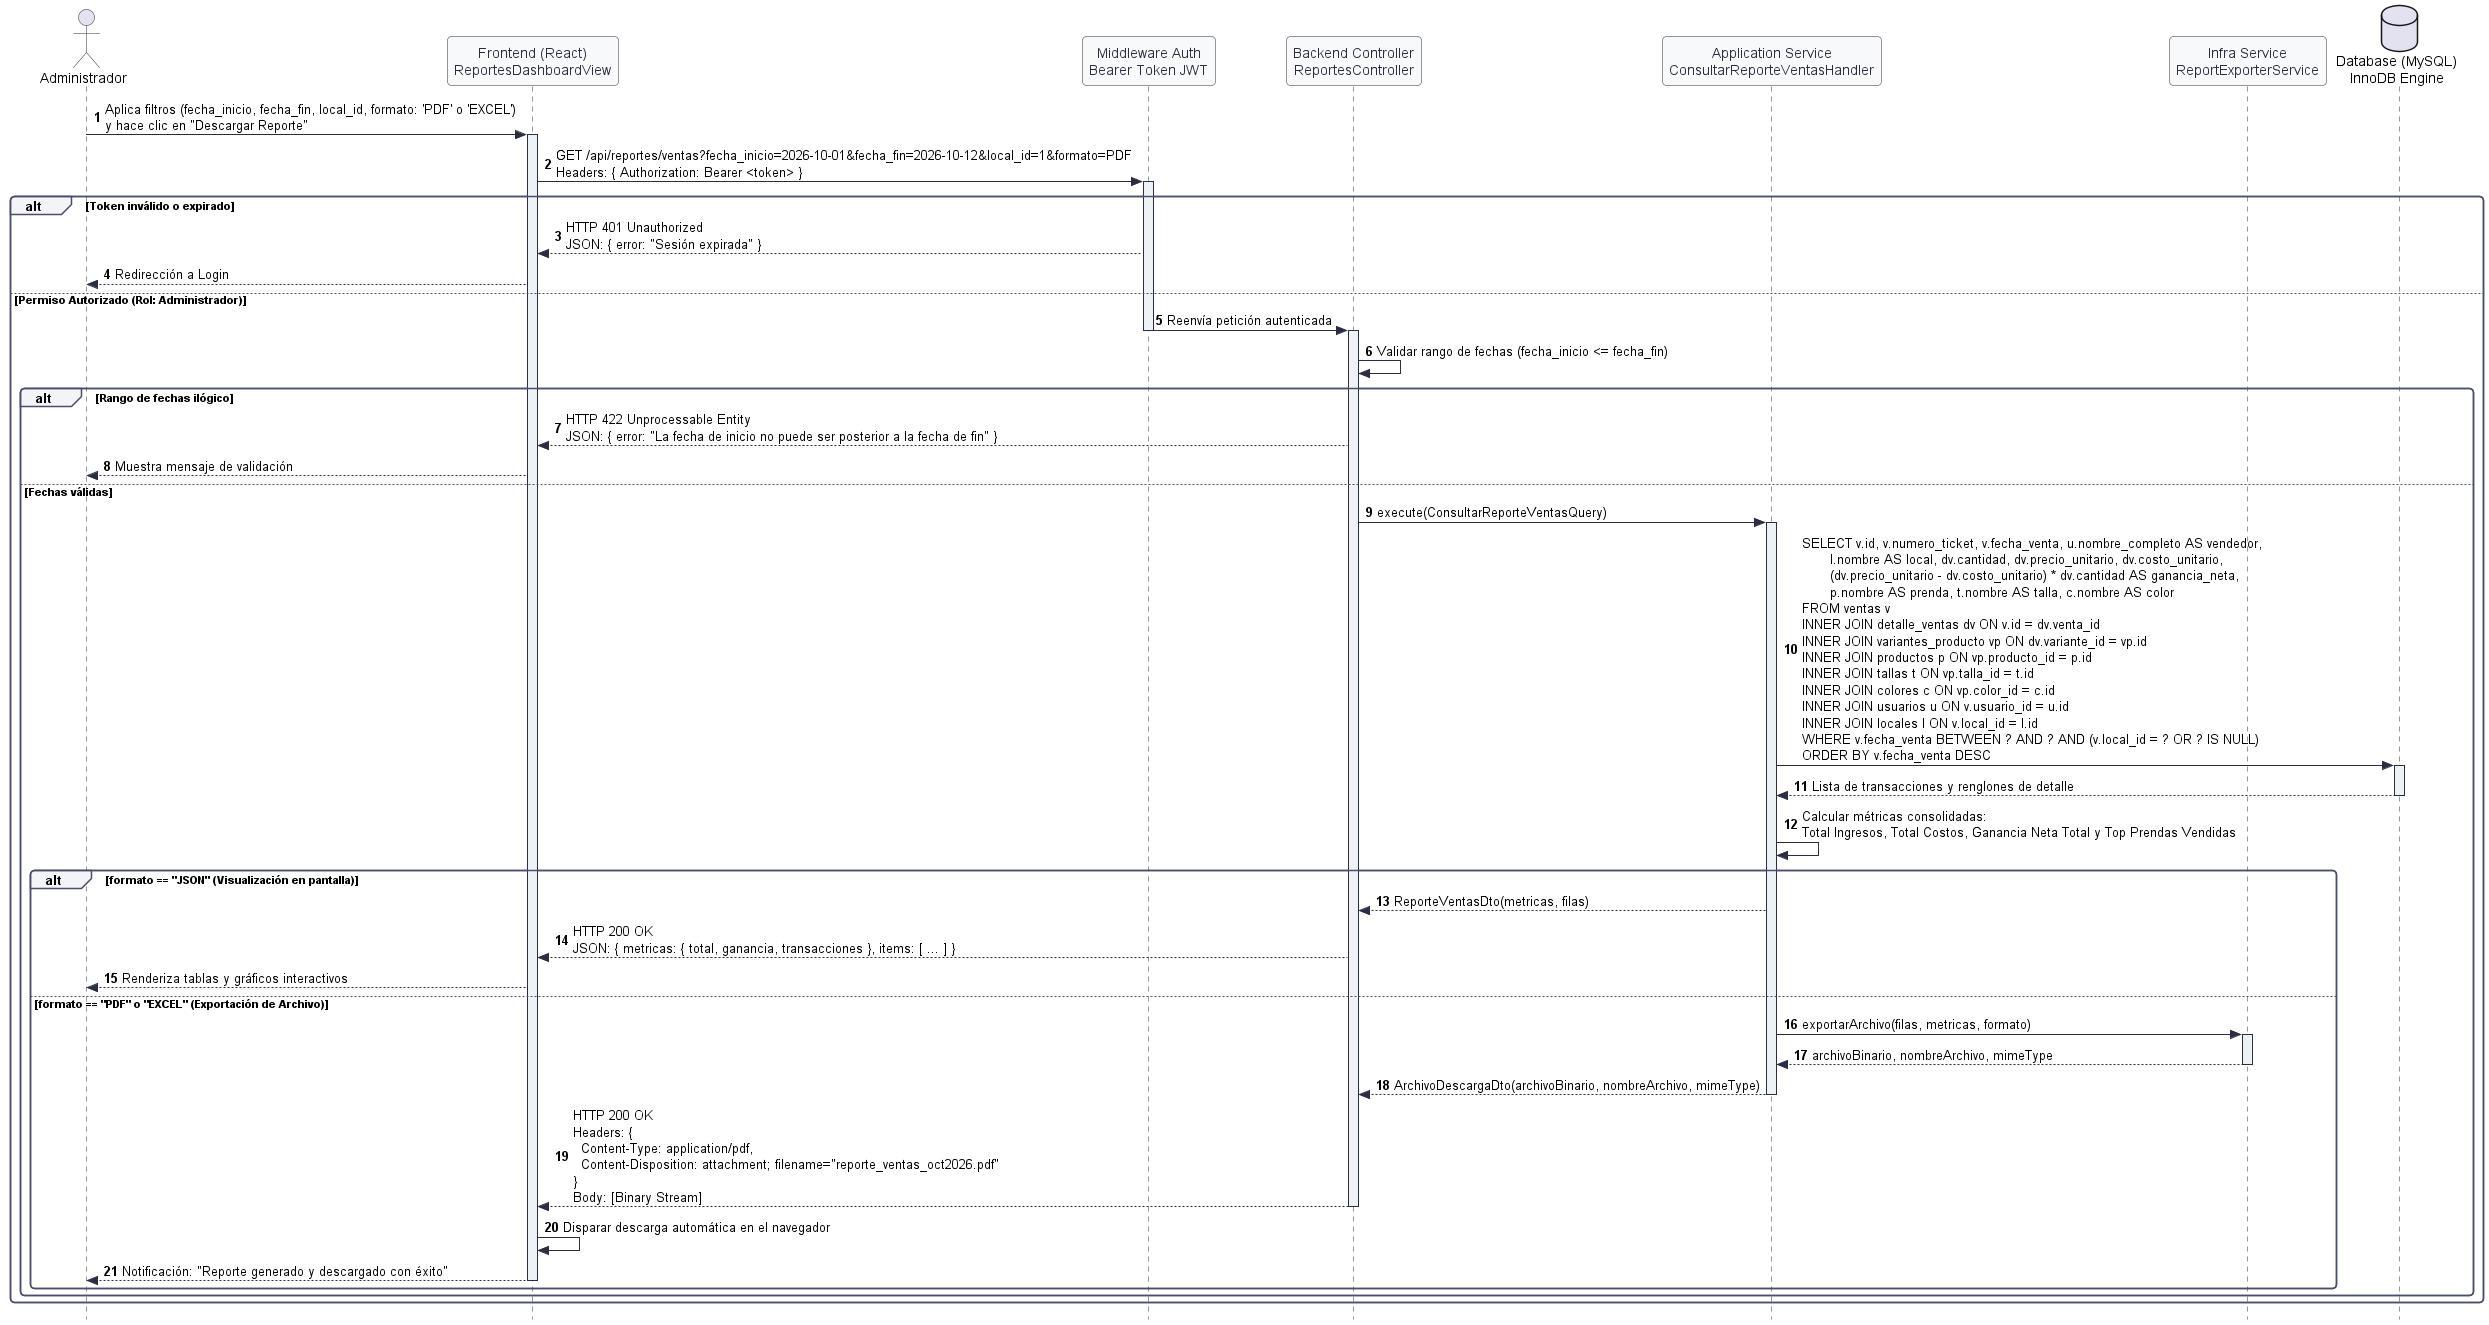
\includegraphics[width=0.92\textwidth]{ds_05_generacion_reporte_ventas.png}
\caption{Diagrama de Secuencia DS-05: Generación y Exportación de Reportes de Ventas}
\label{fig:ds_05}
\end{figure}

\subsection{Anulación Supervisada de Venta (DS-08)}
La anulación es un privilegio exclusivo del Administrador (\texttt{RF-53}). Requiere reautenticación con contraseña y un motivo formal. El servicio verifica que la venta no esté previamente anulada, actualiza el estado a \texttt{'ANULADA'}, reincorpora las unidades vendidas al stock del local correspondiente e inserta un registro inmutable en la tabla \texttt{auditoria}.

\chapter{Arquitectura del Software (Clean Architecture + CQRS + OWASP)}

\section{Patrón Arquitectónico: Clean Architecture en 4 Capas}
Para garantizar la mantenibilidad, escalabilidad y la independencia de frameworks o tecnologías externas, \textbf{SYSELL Web v2.0} adopta los principios de \textbf{Clean Architecture} propuestos por Robert C. Martin. La arquitectura se organiza en cuatro capas concéntricas con una regla de dependencia estricta: \textit{las dependencias del código apuntan únicamente hacia el interior}, asegurando que las reglas de negocio nunca dependan de bibliotecas, bases de datos o interfaces de usuario.

\begin{figure}[H]
\centering
\begin{tikzpicture}[
    scale=0.92, every node/.style={transform shape},
    cPres/.style={rectangle, draw=blue!80!black, fill=blue!10, rounded corners=6pt, line width=1.2pt, minimum width=12.8cm, minimum height=5.2cm},
    cInfra/.style={rectangle, draw=purple!80!black, fill=purple!10, rounded corners=5pt, line width=1.2pt, minimum width=10.6cm, minimum height=3.9cm},
    cApp/.style={rectangle, draw=cyan!80!black, fill=cyan!10, rounded corners=4pt, line width=1.2pt, minimum width=8.4cm, minimum height=2.7cm},
    cDom/.style={rectangle, draw=green!70!black, fill=green!15, rounded corners=3pt, line width=1.2pt, minimum width=6.2cm, minimum height=1.6cm, align=center}
]

% Capa 4: Presentacion
\node[cPres] (pres) at (0, 0) {};
\node[anchor=north, font=\bfseries\small, text=blue!80!black] at (0, 2.5) {Capa de Presentación (Controladores REST Laravel, React 18 SPA, Web Mobile)};

% Capa 3: Infraestructura
\node[cInfra] (infra) at (0, -0.3) {};
\node[anchor=north, font=\bfseries\small, text=purple!80!black] at (0, 1.6) {Capa de Infraestructura (MySQL 8.0, Sanctum Auth, Repositorios Eloquent, PDF/Excel)};

% Capa 2: Aplicacion
\node[cApp] (app) at (0, -0.6) {};
\node[anchor=north, font=\bfseries\small, text=cyan!80!black] at (0, 0.7) {Capa de Aplicación (Commands, Queries, Application Services, Interfaces)};

% Capa 1: Dominio
\node[cDom] (dom) at (0, -0.9) {\textbf{Capa de Dominio (Núcleo Puro)}\\\scriptsize Entidades (Prenda, Variante, Venta, Usuario), Value Objects (SKU, Moneda)\\\scriptsize Reglas Invariantes de Negocio (Sin dependencias externas)};

% Regla de Dependencia
\draw[-{Stealth[length=2.5mm]}, line width=1.8pt, red!80!black] (-5.8, -2.1) -- (-5.8, 2.1)
    node[midway, left=2pt, rotate=90, font=\scriptsize\bfseries, text=red!80!black] {Regla de Dependencia (Hacia el Dominio)};

\end{tikzpicture}
\caption{Diagrama de Cuatro Capas Concéntricas de Clean Architecture en SYSELL Web}
\label{fig:clean_architecture}
\end{figure}

\subsection{Descripción de Responsabilidades por Capa}
\begin{itemize}
    \item \textbf{Capa de Dominio:} Contiene la lógica esencial del negocio de ropa masculina. Las entidades como \texttt{Producto} o \texttt{Variante} hacen cumplir reglas invariantes (por ejemplo, el precio de venta debe ser estrictamente mayor a cero y el SKU debe cumplir con la nomenclatura \texttt{[CAT]-[MOD]-[COL]-[TAL]}). Esta capa no contiene dependencias de Laravel, React ni SQL.
    \item \textbf{Capa de Aplicación:} Implementa los casos de uso del sistema. Orquesta el flujo de información utilizando interfaces de repositorios abstractas (\texttt{IProductoRepository}, \texttt{IVentaRepository}), sin conocer si los datos se guardan en MySQL, PostgreSQL o memoria.
    \item \textbf{Capa de Infraestructura:} Implementa las interfaces de persistencia y servicios externos. Aquí residen las consultas SQL a MySQL 8.0, el almacenamiento de fotografías y el despacho de mensajes.
    \item \textbf{Capa de Presentación:} Provee los endpoints HTTP/JSON y renderiza los componentes interactivos de la interfaz web responsiva (Mobile-first).
\end{itemize}

\section{Patrón CQRS (Command Query Responsibility Segregation)}
Para optimizar el rendimiento y clarificar las intenciones transaccionales, se aplicó el patrón \textbf{CQRS}, separando conceptual y operativamente las acciones del sistema en dos modelos de ejecución:

\begin{figure}[H]
\centering
\begin{tikzpicture}[
    scale=0.88, every node/.style={transform shape},
    boxC/.style={rectangle, draw=red!70!black, fill=red!10, rounded corners=3pt, thick, align=center, minimum width=4.0cm, minimum height=1.1cm, font=\small},
    boxQ/.style={rectangle, draw=blue!70!black, fill=blue!10, rounded corners=3pt, thick, align=center, minimum width=4.0cm, minimum height=1.1cm, font=\small},
    dbNode/.style={cylinder, shape border rotate=90, draw=purple!80!black, fill=purple!15, aspect=0.3, minimum width=2.4cm, minimum height=2.4cm, align=center, font=\small\bfseries},
    flow/.style={thick, -{Stealth[length=2.2mm]}}
]

\node[rectangle, draw=gray!70, fill=gray!10, rounded corners=3pt, minimum width=2.8cm, minimum height=3.0cm, align=center] (client) at (-5.2, 0) {\textbf{Cliente Web / POS}\\\scriptsize (Peticiones HTTP)};

\node[boxC] (cmd) at (0, 1.4) {\textbf{Command Bus (Escritura)}\\\scriptsize Transacciones ACID (Venta, Ajuste)};
\node[boxQ] (qry) at (0, -1.4) {\textbf{Query Bus (Lectura)}\\\scriptsize Consultas Directas / Vistas};

\node[dbNode] (db) at (5.2, 0) {Base de Datos\\MySQL 8.0\\(3FN)};

% Flujos de Comandos
\draw[flow, red!80!black] (client.north) |- node[pos=0.72, above=2pt, font=\scriptsize\bfseries] {POST / PUT (Comandos)} (cmd.west);
\draw[flow, red!80!black] (cmd.east) -| node[pos=0.28, above=2pt, font=\scriptsize\bfseries] {Mutaciones ACID} (db.north);

% Flujos de Consultas
\draw[flow, blue!80!black] (client.south) |- node[pos=0.72, below=2pt, font=\scriptsize\bfseries] {GET (Catálogo, Reportes)} (qry.west);
\draw[flow, blue!80!black] (db.south) -| node[pos=0.28, below=2pt, font=\scriptsize\bfseries] {Proyecciones Optimizadas} (qry.east);

\end{tikzpicture}
\caption{Segregación Operativa de Comandos y Consultas con el Patrón CQRS}
\label{fig:cqrs_pattern}
\end{figure}

\begin{enumerate}
    \item \textbf{Commands (Comandos de Escritura):} Mutan el estado del sistema. Modifican datos, disparan transacciones ACID y retornan confirmación o IDs (ej. creación de prendas, confirmación de venta POS, anulación y ajustes de Kardex).
    \item \textbf{Queries (Consultas de Lectura):} Solo leen datos sin alterar el estado. Están optimizadas con proyecciones SQL directas y paginación (ej. consulta del catálogo web, stock por sucursal y reportería gerencial).
\end{enumerate}

\section{Seguridad Web (OWASP Top 10) y Autenticación Híbrida}
El sistema adopta las directrices de seguridad de \textbf{OWASP Top 10} para mitigar vulnerabilidades comunes:

\begin{table}[H]
\centering
\small
\begin{tabularx}{\textwidth}{>{\bfseries}p{3.8cm} >{\raggedright}p{4.8cm} Y}
\toprule
\textbf{Vulnerabilidad OWASP} & \textbf{Mecanismo de Protección en SYSELL} & \textbf{Implementación Técnica} \\
\midrule
A01: Broken Access Control & Control RBAC estricto a nivel de Middleware en cada endpoint API. & Roles \texttt{ADMINISTRADOR} y \texttt{VENDEDOR} evaluados en servidor antes de procesar la solicitud. \\
\addlinespace
A02: Cryptographic Failures & Cifrado unidireccional y canales seguros de transporte. & Contraseñas con hash Bcrypt (cost 12), forzando HTTPS con encabezados HSTS en producción. \\
\addlinespace
A03: Injection (SQLi) & Consultas parametrizadas obligatorias. & Uso exclusivo del Query Builder / Eloquent ORM; prohibido el concatenado de variables crudas en SQL. \\
\addlinespace
A07: Identification Failures & Bloqueo preventivo de cuentas y rate limiting. & Bloqueo automático al tercer fallo consecutivo (\texttt{RF-06}) y acelerador de retardo en reintentos. \\
\bottomrule
\end{tabularx}
\caption{Matriz de mitigación de vulnerabilidades de seguridad OWASP Top 10}
\label{tab:owasp_security}
\end{table}

\subsection{Estrategia Dual de Autenticación con Laravel Sanctum}
Para armonizar la seguridad del navegador con las necesidades de las terminales físicas de punto de venta:
\begin{enumerate}
    \item \textbf{Modo SPA Web (Navegador):} Utiliza cookies \texttt{HttpOnly}, \texttt{Secure} y \texttt{SameSite=Lax} con validación de token CSRF para el portal web administrativo y la tienda React, protegiendo las credenciales contra ataques de robo de sesión (XSS).
    \item \textbf{Modo API Token (Terminal POS / Sincronización):} Utiliza \textit{Bearer Tokens} (Personal Access Tokens) en el encabezado HTTP \texttt{Authorization} para permitir la operación en terminales de caja dedicadas y el envío de lotes de sincronización offline (\texttt{CU-10}).
\end{enumerate}

\chapter{Modelo de Datos Relacional (MySQL 8.0 en 3FN) e Infraestructura}

\section{Diseño Conceptual y Normalización en Tercera Forma Normal (3FN)}
El modelo de base de datos de \textbf{SYSELL Web v2.0} fue diseñado bajo el motor relacional **MySQL 8.0** con almacenamiento **InnoDB**, aplicando rigurosamente los principios de normalización relacional hasta la **Tercera Forma Normal (3FN)**:
\begin{itemize}
    \item \textbf{Primera Forma Normal (1FN):} Se eliminaron grupos repetitivos y atributos multivaluados. Cada celda contiene valores atómicos.
    \item \textbf{Segunda Forma Normal (2FN):} En tablas con claves compuestas (como \texttt{inventario} o \texttt{variantes\_producto}), todos los atributos no clave dependen funcionalmente de la totalidad de la clave primaria.
    \item \textbf{Tercera Forma Normal (3FN):} No existen dependencias transitivas; ningún atributo no clave depende de otro atributo no clave. Por ejemplo, los datos descriptivos de colores y tallas residen en sus propias tablas maestras cerradas (\texttt{colores}, \texttt{tallas}) y no incrustados en la tabla de productos.
\end{itemize}

\section{Catálogo y Estructura de las 17 Tablas del Sistema}
El modelo relacional abarca 17 entidades organizadas en 5 grupos funcionales:

\begin{table}[H]
\centering
\small
\begin{tabularx}{\textwidth}{c l l p{6.5cm}}
\toprule
\textbf{N$^\circ$} & \textbf{Tabla Relacional} & \textbf{Clave Primaria} & \textbf{Propósito y Rol en el Sistema} \\
\midrule
1 & \texttt{locales} & \texttt{id (BIGINT)} & Registro de las dos sucursales físicas (San Martín y Bolognesi). \\
2 & \texttt{usuarios} & \texttt{id (BIGINT)} & Cuentas de acceso, credenciales Bcrypt, intentos y rol RBAC. \\
3 & \texttt{categorias} & \texttt{id (BIGINT)} & Catálogo cerrado de familias de prendas (Camisas, Polos, etc.). \\
4 & \texttt{marcas} & \texttt{id (BIGINT)} & Catálogo cerrado de marcas comerciales de confección. \\
5 & \texttt{tallas} & \texttt{id (BIGINT)} & Catálogo maestro de tallas alfabéticas y numéricas (RF-74). \\
6 & \texttt{colores} & \texttt{id (BIGINT)} & Catálogo de colores con código hexadecimal para vista web. \\
7 & \texttt{metodos\_pago} & \texttt{id (BIGINT)} & Medios de cobro habilitados (Efectivo, Tarjetas, Yape, Plin). \\
8 & \texttt{productos} & \texttt{id (BIGINT)} & Prenda base masculina con código de modelo y precios oficiales. \\
9 & \texttt{imagenes\_producto} & \texttt{id (BIGINT)} & Galería de fotos en alta definición por prenda (RF-69). \\
10 & \texttt{variantes\_producto}& \texttt{id (BIGINT)} & Combinación física vendible de Talla + Color con código SKU único. \\
11 & \texttt{inventario} & \texttt{id (BIGINT)} & Existencias físicas independientes y stock mínimo por local. \\
12 & \texttt{ventas} & \texttt{id (BIGINT)} & Encabezado de transacción comercial con número de ticket único. \\
13 & \texttt{detalle\_ventas} & \texttt{id (BIGINT)} & Desglose de prendas, precios históricos y subtotales por venta. \\
14 & \texttt{pagos\_venta} & \texttt{id (BIGINT)} & Liquidación multitendencia de medios de pago combinados. \\
15 & \texttt{ajustes\_inventario}& \texttt{id (BIGINT)} & Asientos auditables de Kardex (ingresos, mermas, correcciones). \\
16 & \texttt{reportes\_configuracion}& \texttt{id (BIGINT)} & Parámetros JSON y programaciones de reportes gerenciales. \\
17 & \texttt{auditoria} & \texttt{id (BIGINT)} & Bitácora inmutable de eventos críticos con snapshot JSON (HU-18). \\
\bottomrule
\end{tabularx}
\caption{Catálogo de las 17 tablas relacionales normalizadas en MySQL 8.0}
\label{tab:tablas_bd}
\end{table}

\section{Reglas de Integridad Referencial y Restricciones Transaccionales}
Para salvaguardar la integridad de los datos ante eliminaciones accidentales o actualizaciones:
\begin{itemize}
    \item \textbf{Protección contra orfandad comercial (\texttt{ON DELETE RESTRICT}):} Si una prenda o variante registra ventas históricas en \texttt{detalle\_ventas}, la base de datos bloquea cualquier intento de borrado físico en \texttt{productos} o \texttt{variantes\_producto}. La baja debe procesarse mediante borrado lógico (\texttt{activo = 0}).
    \item \textbf{Eliminación en cascada controlada (\texttt{ON DELETE CASCADE}):} Si se da de baja una prenda base que no registra ventas, sus variantes e imágenes asociadas en \texttt{imagenes\_producto} se suprimen automáticamente sin dejar registros basura.
    \item \textbf{Unicidad Compuesta:} Se aplican restricciones \texttt{UNIQUE} compuestas:
    \begin{itemize}
        \item \texttt{(producto\_id, talla\_id, color\_id)} en \texttt{variantes\_producto} para impedir variantes duplicadas de una misma prenda.
        \item \texttt{(local\_id, variante\_id)} en \texttt{inventario} para asegurar un único registro de balance de existencias por tienda.
    \end{itemize}
\end{itemize}

\section{Scripts SQL Ejecutables y Datos Semilla}
La estructura física de la base de datos se encuentra totalmente codificada y versionada en el repositorio:
\begin{itemize}
    \item \texttt{database/schema.sql}: Script DDL con la creación de tablas, índices y llaves foráneas.
    \item \texttt{database/seeds.sql}: Datos iniciales para locales, catálogos maestros cerrados de tallas, colores, marcas y usuario administrador de prueba.
\end{itemize}
El esquema completo puede ser levantado de forma automática mediante contenedores Docker con el comando \texttt{docker compose up -d}.

\chapter{Aseguramiento de Calidad y Pruebas del Software}
\label{cap:calidad_pruebas}

\section{Estrategia de Calidad y Marco Normativo IEEE 829 / ISTQB}
El aseguramiento de calidad del software (SQA) en el proyecto Tienda Machi's se rige bajo los lineamientos del estándar internacional \textbf{IEEE 829} (Standard for Software and System Test Documentation) y las directrices metodológicas del \textbf{ISTQB} (International Software Testing Qualifications Board). En respuesta a la interrogante formativa de la cátedra:
\begin{quote}
\textit{«¿Cómo demuestro fehacientemente que se cumplió el requerimiento? Respuesta: Mediante criterios de aceptación medibles y casos de prueba empíricos».}
\end{quote}

A diferencia del proyecto heredado (Legacy v1.0), el cual carecía por completo de especificaciones de prueba formales, matrices de validación o criterios de aceptación estructurados, la versión 2.0 define un conjunto exhaustivo de \textbf{77 Casos de Prueba (CP-01 a CP-77)}, estableciendo una correspondencia unívoca y bidireccional ($1:1$) con los 77 Requisitos Funcionales aprobados.

\begin{figure}[H]
\centering
\begin{tikzpicture}[
    scale=0.9, every node/.style={transform shape},
    pyrLevel/.style={trapezium, trapezium left angle=70, trapezium right angle=70, draw=primaryblue!80!black, line width=1pt, align=center, font=\small}
]

% Nivel 3: Pruebas E2E y Aceptacion
\node[pyrLevel, fill=red!15, draw=red!70!black, minimum width=4.5cm, minimum height=1.0cm] at (0, 2.4) {\textbf{Nivel E2E y Aceptación}\\\scriptsize 77 Casos de Prueba Formales (CP-01 a CP-77) y Validación UI};

% Nivel 2: Pruebas de Integracion
\node[pyrLevel, fill=orange!15, draw=orange!70!black, minimum width=8.5cm, minimum height=1.0cm] at (0, 1.2) {\textbf{Nivel de Integración y Servicios}\\\scriptsize Transacciones ACID, Descuento atómico, Bloqueo de 3 intentos, Middlewares RBAC};

% Nivel 1: Pruebas Unitarias
\node[pyrLevel, fill=green!15, draw=green!70!black, minimum width=12.5cm, minimum height=1.0cm] at (0, 0.0) {\textbf{Nivel Unitario (Lógica Pura de Dominio)}\\\scriptsize Validación de SKU, Catálogos Maestros Cerrados, Cálculo de Totales y Vuelto};

\end{tikzpicture}
\caption{Pirámide de Pruebas y Aseguramiento de Calidad en SYSELL Web (IEEE 829 / ISTQB)}
\label{fig:piramide_pruebas}
\end{figure}

\section{Estructura Estándar de los Casos de Prueba}
Cada caso de prueba diseñado en la especificación formal cuenta con los siguientes atributos:
\begin{enumerate}
    \item \textbf{Identificador Único:} Código correlativo estandarizado \texttt{CP-XX}.
    \item \textbf{Requerimiento Trazado:} Código \texttt{RF-XX} y denominación funcional.
    \item \textbf{Tipo de Prueba:} Validación de interfaz (UI), Lógica de negocio backend, Validación de límites (BVA), Prueba negativa / robustez o Seguridad (RBAC / OWASP).
    \item \textbf{Precondiciones y Datos de Entrada:} Estado del sistema, roles requeridos y payloads de entrada.
    \item \textbf{Procedimiento de Ejecución:} Secuencia cronológica y determinista de pasos ejecutados por el usuario o cliente HTTP.
    \item \textbf{Resultado Esperado y Criterios Verificados:} Comportamiento verificable de la interfaz, códigos de respuesta HTTP (e.g., \texttt{200 OK}, \texttt{201 Created}, \texttt{403 Forbidden}, \texttt{422 Unprocessable Entity}) y mutaciones de persistencia en base de datos.
    \item \textbf{Estado de Verificación:} Trazado como diseñado, listo para ejecución en el pipeline de CI/CD.
\end{enumerate}

\section{Distribución Modular de los Casos de Prueba}
Los 77 casos de prueba se distribuyen equitativamente en los 5 módulos arquitectónicos del sistema:

\begin{table}[H]
\centering
\small
\begin{tabularx}{\textwidth}{|>{\bfseries\raggedright}p{4.2cm}|>{\centering}p{4cm}|>{\centering}p{3.5cm}|Z|}
\hline
\textbf{Módulo del Sistema} & \textbf{Requisitos Trazados} & \textbf{Rango Casos de Prueba} & \textbf{Total} \\ \hline
M1: Autenticación y Seguridad & RF-01 al RF-14, RF-73 & CP-01 al CP-14, CP-73 & 15 CP \\ \hline
M2: Gestión de Inventario & RF-15 al RF-39, RF-74, RF-75, RF-77 & CP-15 al CP-39, CP-74, CP-75, CP-77 & 28 CP \\ \hline
M3: Registro de Ventas (POS) & RF-40 al RF-55, RF-76 & CP-40 al CP-55, CP-76 & 17 CP \\ \hline
M4: Reportes y Análisis Gerencial & RF-56 al RF-66 & CP-56 al CP-66 & 11 CP \\ \hline
M5: Catálogo Digital Web & RF-67 al RF-72 & CP-67 al CP-72 & 6 CP \\ \hline
\textbf{TOTAL GENERAL} & \textbf{RF-01 al RF-77} & \textbf{CP-01 al CP-77} & \textbf{77 CP} \\ \hline
\end{tabularx}
\caption{Distribución de Casos de Prueba por Módulo del Sistema}
\label{tab:distribucion_cp}
\end{table}

\section{Especificación de Casos de Prueba Críticos por Módulo}
A continuación, se documenta una selección representativa de casos de prueba que cubren los flujos críticos de seguridad, consistencia transaccional y reglas de negocio del sistema:

\subsection{Módulo 1: Autenticación y Control de Acceso (CP-01 a CP-14, CP-73)}
\begin{table}[H]
\centering
\small
\begin{tabularx}{\textwidth}{|>{\ttfamily\centering}p{1.4cm}|>{\raggedright\bfseries}p{3.4cm}|>{\raggedright}p{2.2cm}|Y|}
\hline
\textbf{ID} & \textbf{RF / Propósito} & \textbf{Tipo} & \textbf{Procedimiento y Resultado Esperado} \\ \hline
CP-01 & RF-01: Solicitar usuario & Validación UI & Formulario de Login. Se deja campo usuario vacío e ingresa clave. \textit{Resultado:} Formulario bloquea submit y alerta campo obligatorio. \\ \hline
CP-04 & RF-04: Validar credenciales & Backend API & Petición POST a \texttt{/api/auth/login}. \textit{Resultado:} Backend compara hash bcrypt contra BD y genera token Sanctum válido si coincide. \\ \hline
CP-06 & RF-06: Bloqueo por 3 intentos & Seguridad & 3 accesos consecutivos con password errónea. \textit{Resultado:} El 3er intento conmuta estado a \texttt{bloqueado} e incrementa \texttt{intentos\_fallidos = 3}. \\ \hline
CP-08 & RF-08: Restricción RBAC & Seguridad RBAC & Vendedor autenticado intenta acceder a \texttt{/api/reportes/gerenciales}. \textit{Resultado:} Middleware responde HTTP 403 Forbidden. \\ \hline
CP-14 & RF-14: Desbloqueo de cuenta & Seguridad & Administrador selecciona colaborador bloqueado y ejecuta desbloqueo. \textit{Resultado:} Estado cambia a \texttt{activo} y contador se restablece a 0. \\ \hline
\end{tabularx}
\caption{Casos de Prueba Clave --- Módulo de Autenticación y Seguridad}
\label{tab:cp_modulo1}
\end{table}

\subsection{Módulo 2: Gestión de Inventario Multi-Tienda (CP-15 a CP-39, CP-74, CP-75, CP-77)}
\begin{table}[H]
\centering
\small
\begin{tabularx}{\textwidth}{|>{\ttfamily\centering}p{1.4cm}|>{\raggedright\bfseries}p{3.4cm}|>{\raggedright}p{2.2cm}|Y|}
\hline
\textbf{ID} & \textbf{RF / Propósito} & \textbf{Tipo} & \textbf{Procedimiento y Resultado Esperado} \\ \hline
CP-15 & RF-15: Registrar prenda & Funcional & Envío de datos de prenda, categoría y tallas iniciales. \textit{Resultado:} Prenda creada con código correlativo en BD. \\ \hline
CP-23 & RF-23: Alerta de stock mínimo & Lógica Negocio & El stock disponible de una talla desciende por debajo de 3 unidades. \textit{Resultado:} Se emite flag \texttt{bajo\_stock = true} en dashboard. \\ \hline
CP-33 & RF-33: Traslado entre locales & Transaccional & Solicitud de traslado de 5 unidades de Local A a Local B. \textit{Resultado:} Descuento en origen, incremento en destino bajo transacción ACID única. \\ \hline
CP-35 & RF-35: Rechazo sobregiro & Límite / Negativa & Intento de traslado de 10 unidades cuando el stock físico es de 4 unidades. \textit{Resultado:} Rechazo inmediato con código HTTP 422 y rollback. \\ \hline
CP-77 & RF-77: Desglose por variante & Integridad & Consulta de SKU por variantes múltiples. \textit{Resultado:} La matriz cartesiana talla/color/local cuadra exactamente con el total. \\ \hline
\end{tabularx}
\caption{Casos de Prueba Clave --- Módulo de Inventario}
\label{tab:cp_modulo2}
\end{table}

\subsection{Módulo 3: Punto de Venta y Transacciones POS (CP-40 a CP-55, CP-76)}
\begin{table}[H]
\centering
\small
\begin{tabularx}{\textwidth}{|>{\ttfamily\centering}p{1.4cm}|>{\raggedright\bfseries}p{3.4cm}|>{\raggedright}p{2.2cm}|Y|}
\hline
\textbf{ID} & \textbf{RF / Propósito} & \textbf{Tipo} & \textbf{Procedimiento y Resultado Esperado} \\ \hline
CP-40 & RF-40: Apertura de caja & Financiero & Cajero ingresa monto inicial de apertura. \textit{Resultado:} Registro de apertura persistido con timestamp y estado \texttt{abierta}. \\ \hline
CP-44 & RF-44: Búsqueda de prenda & Rendimiento UI & Escaneo de código de barras o búsqueda de texto. \textit{Resultado:} Resultados desplegados en pantalla en menos de 300 ms. \\ \hline
CP-49 & RF-49: Descuento atómico & Transaccional & Confirmación de venta con 2 ítems. \textit{Resultado:} Stock físico decrementado atómicamente; no se permiten carreras concurrentes. \\ \hline
CP-53 & RF-53: Arqueo ciego & Auditoría & Cajero declara efectivo al cierre sin ver total del sistema. \textit{Resultado:} Sistema calcula sobrante/faltante y congela operaciones. \\ \hline
CP-76 & RF-76: Multi-método de pago & Lógica Negocio & Pago dividido: S/. 100 en Efectivo y S/. 50 con billetera digital Yape. \textit{Resultado:} Ambas transacciones registradas cuadrando el total exacto. \\ \hline
\end{tabularx}
\caption{Casos de Prueba Clave --- Módulo POS y Facturación}
\label{tab:cp_modulo3}
\end{table}

\section{Pruebas de Seguridad y Resiliencia (OWASP)}
Adicionalmente a las pruebas funcionales, se diseñaron pruebas específicas de robustez y seguridad basadas en el estándar OWASP:
\begin{itemize}
    \item \textbf{Inyección SQL (OWASP A03):} Verificación de que todos los endpoints de consulta utilicen PDO con parámetros vinculados (Prepared Statements), evitando concatenación directa de cadenas.
    \item \textbf{Cross-Site Scripting (XSS - OWASP A03):} Saneamiento y escape automático de caracteres especiales en campos de texto antes de su renderizado en clientes Vue.js/React.
    \item \textbf{Control de Acceso Quebrantado (BOLA / IDOR - OWASP A01):} Verificación de que un usuario con rol Vendedor en Local A no pueda consultar o alterar las ventas del Local B modificando identificadores en URLs.
\end{itemize}

El conjunto de pruebas estructurado garantiza un nivel de madurez técnica certificable, eliminando la incertidumbre en la aceptación del producto software final.

\chapter{Gestión Ágil del Proyecto: Sprints, Backlog y EDT / WBS}
\label{cap:gestion_proyecto}

\section{Estructura del Product Backlog e Historias de Usuario}
El desarrollo del proyecto se gestionó bajo el marco de trabajo ágil Scrum, articulado mediante un \textbf{Product Backlog} compuesto por \textbf{18 Historias de Usuario (HU)} distribuidas en 7 Épicas de negocio, sumando un esfuerzo total estimado de \textbf{94 Puntos de Historia (Story Points - SP)} calculados mediante la técnica de \textit{Planning Poker} con escala Fibonacci.

\begin{table}[H]
\centering
\small
\caption{Resumen de Épicas y Distribución de Historias de Usuario}
\label{tab:epicas_backlog}
\begin{tabular}{|l|c|c|l|}
\hline
\textbf{Épica} & \textbf{Cant. HU} & \textbf{Puntos (SP)} & \textbf{Objetivo de Negocio} \\ \hline
EP-01: Autenticación y Seguridad & 3 HU & 13 SP & Control de acceso y gobierno RBAC. \\ \hline
EP-02: Catálogo e Inventario Multi-Tienda & 4 HU & 22 SP & Control de prendas, tallas, colores y stock físico. \\ \hline
EP-03: Logística y Traslados Internos & 2 HU & 13 SP & Transferencias atómicas entre sucursales. \\ \hline
EP-04: Punto de Venta (POS) y Caja & 4 HU & 21 SP & Apertura/cierre de caja, facturación y cobros. \\ \hline
EP-05: Analítica y Reportes Gerenciales & 2 HU & 11 SP & Métricas financieras, rotación y alertas. \\ \hline
EP-06: Catálogo Web de Exhibición & 2 HU & 8 SP & Vitrina digital para clientes finales sin pasarela. \\ \hline
EP-07: Infraestructura y DevOps & 1 HU & 6 SP & Contenedores Docker y automatización CI. \\ \hline
\textbf{TOTAL GENERAL} & \textbf{18 HU} & \textbf{94 SP} & \textbf{Alcance Completo v2.0} \\ \hline
\end{tabular}
\end{table}

\section{Criterios de Preparación (DoR) y Criterios de Finalización (DoD)}
Para asegurar un flujo continuo y predecible de entrega de valor, el equipo \textit{Pollitos Design} acordó formalmente los siguientes criterios:

\subsection{Definition of Ready (DoR - Criterio de Preparación)}
Una Historia de Usuario únicamente puede ingresar al Sprint Backlog si cumple con:
\begin{enumerate}
    \item Formato estándar: \textit{«Como [Rol], quiero [Acción/Capacidad] para [Beneficio de Negocio]»}.
    \item Criterios de aceptación detallados y verificables bajo la sintaxis Given-When-Then (Gherkin).
    \item Dependencias arquitectónicas resueltas y estimación acordada por el equipo técnico.
    \item Mockups de interfaz o contratos de API definidos si la historia involucra cambios de presentación.
\end{enumerate}

\subsection{Definition of Done (DoD - Criterio de Terminado)}
Un incremento de software se considera potencialmente entregable únicamente cuando:
\begin{enumerate}
    \item Código fuente implementado y refactorizado respetando las 4 capas de Clean Architecture.
    \item Pruebas unitarias y de integración asociadas ejecutadas con resultado exitoso ($100\%$ pass).
    \item Código libre de vulnerabilidades críticas y analizado mediante linters estáticos en CI.
    \item Migraciones de base de datos ejecutables hacia adelante y hacia atrás (\texttt{up} y \texttt{down}).
    \item Documentación técnica de endpoints y diagramas de secuencia sincronizados.
    \item Merge a la rama principal mediante Pull Request revisado por al menos un par técnico.
\end{enumerate}

\section{Planificación y Ejecución de los 4 Sprints}
El ciclo de desarrollo se estructuró en cuatro iteraciones de dos semanas de duración cada una:

\subsection{Sprint 1: Fundaciones, Seguridad y Modelo de Dominio (24 SP)}
\textbf{Objetivo:} Construir el núcleo arquitectónico, la base de datos relacional normalizada y el subsistema de autenticación con gobierno de roles.
\begin{itemize}
    \item \textbf{HU-01:} Autenticación segura con bloqueo por 3 intentos fallidos (5 SP).
    \item \textbf{HU-02:} Asignación de roles de usuario (RBAC) y control de perfiles (5 SP).
    \item \textbf{HU-03:} Gestión administrativa de colaboradores y auditoría de accesos (8 SP).
    \item \textbf{HU-18:} Infraestructura de contenedorización Docker y orquestación de servicios (6 SP).
\end{itemize}

\subsection{Sprint 2: Gestión de Inventario Multi-Tienda y Traslados (26 SP)}
\textbf{Objetivo:} Implementar el catálogo de prendas con variantes ortogonales de talla/color y el mecanismo transaccional de transferencias entre locales.
\begin{itemize}
    \item \textbf{HU-04:} Registro y parametrización de prendas con variantes por talla y color (8 SP).
    \item \textbf{HU-05:} Actualización de inventario físico y alertas de stock mínimo (5 SP).
    \item \textbf{HU-06:} Consulta de disponibilidad multi-sucursal en tiempo real (5 SP).
    \item \textbf{HU-07:} Solicitud y confirmación atómica de traslados entre sucursales (8 SP).
\end{itemize}

\subsection{Sprint 3: Punto de Venta (POS), Caja y Facturación (24 SP)}
\textbf{Objetivo:} Implementar el flujo transaccional de caja, escaneo de productos, venta multi-método y emisión de comprobantes.
\begin{itemize}
    \item \textbf{HU-08:} Apertura y cierre de caja diaria con arqueo ciego (5 SP).
    \item \textbf{HU-09:} Punto de venta rápido con escaneo de código de barras (8 SP).
    \item \textbf{HU-10:} Registro de venta con múltiples métodos de pago (5 SP).
    \item \textbf{HU-11:} Emisión e impresión de boletas de venta y notas de crédito (6 SP).
\end{itemize}

\subsection{Sprint 4: Analítica Gerencial, Catálogo Web y Despliegue CI/CD (20 SP)}
\textbf{Objetivo:} Desarrollar los módulos analíticos para toma de decisiones, la vitrina web pública y el pipeline automatizado de validación.
\begin{itemize}
    \item \textbf{HU-12:} Reporte de prendas de mayor y menor rotación con gráficos gerenciales (5 SP).
    \item \textbf{HU-13:} Balance financiero de caja y reporte consolidado de utilidades (6 SP).
    \item \textbf{HU-14:} Catálogo digital interactivo responsive para clientes (5 SP).
    \item \textbf{HU-15:} Filtro dinámico de prendas en vitrina web y enlace a WhatsApp (4 SP).
\end{itemize}

\section{Análisis Comparativo y Optimización de la EDT / WBS}
Uno de los hallazgos críticos del diagnóstico de ingeniería de software sobre el proyecto Legacy v1.0 fue la deficiencia estructural de su Estructura de Desglose del Trabajo (EDT / WBS):

\begin{figure}[H]
\centering
\begin{tikzpicture}[
    node distance=1.5cm,
    legacy/.style={rectangle, draw=red!70, fill=red!10, rounded corners, minimum width=4cm, minimum height=0.8cm, align=center},
    modern/.style={rectangle, draw=green!60!black, fill=green!10, rounded corners, minimum width=4cm, minimum height=0.8cm, align=center},
    arrow/.style={thick, -{Stealth}}
]
\node[legacy] (leg) {\textbf{EDT Legacy v1.0}\\(Enfoque Cascada Lineal)};
\node[modern, right=3cm of leg] (mod) {\textbf{EDT Optimizada v2.0}\\(Orientada a Entregables y Capas)};

\draw[arrow, red!80!black, line width=1.5pt] (leg) -- node[above, font=\small\bfseries] {Refactorización} (mod);
\end{tikzpicture}
\caption{Transición Estructural de la EDT del Proyecto}
\label{fig:transicion_edt}
\end{figure}

\begin{table}[H]
\centering
\small
\caption{Matriz de Comparación: EDT Legacy vs. EDT Optimizada v2.0}
\label{tab:comparacion_edt}
\begin{tabular}{|p{3.5cm}|p{5cm}|p{5.5cm}|}
\hline
\textbf{Dimensión de Análisis} & \textbf{EDT Legacy v1.0 (Análisis)} & \textbf{EDT Optimizada v2.0 (Ingeniería)} \\ \hline
\textbf{Enfoque Metodológico} & 5 fases secuenciales en cascada clásica sin ciclos de retroalimentación. & Orientada a entregables de valor con 4 iteraciones incrementales (Sprints). \\ \hline
\textbf{Integridad de Codificación} & Inconsistencia sintáctica: salto arbitrario de \texttt{1.3.1} a \texttt{1.3.1.1} como actividad sin paquete. & Codificación jerárquica estricta según el estándar del Project Management Institute (PMI). \\ \hline
\textbf{Alineación Arquitectónica} & Tareas genéricas («programar módulo») sin separación de responsabilidades. & Tareas estructuradas por capas de Clean Architecture: Dominio, Aplicación, Infraestructura y UI. \\ \hline
\textbf{Calidad y Validación} & Ausencia de aseguramiento formal; no contemplaba casos de prueba IEEE 829. & Paquete específico de SQA con 77 casos de prueba y validación estática en CI/CD. \\ \hline
\textbf{Despliegue y DevOps} & Se limitaba a «instalación en servidor local». & Contenedores Docker Compose, linters de documentación y pipeline GitHub Actions. \\ \hline
\end{tabular}
\end{table}

La EDT v2.0 resultante garantiza trazabilidad total desde las necesidades de negocio del patrocinador de Machi's hasta cada línea de código desplegada en los entornos de ejecución.

\chapter{DevOps, Infraestructura, Ética en IA y Conclusiones}
\label{cap:devops_conclusiones}

\section{Infraestructura como Código y Contenedorización con Docker}
Para mitigar el clásico problema de dispersión de entornos (el antipatrón \textit{«en mi máquina funciona»}) y garantizar la reproducibilidad absoluta del sistema en cualquier estación de trabajo o servidor en la nube, el proyecto implementa Infraestructura como Código mediante \textbf{Docker} y \textbf{Docker Compose}.

\subsection{Topología de Servicios Contenedorizados}
El archivo \texttt{docker-compose.yml} orquesta los servicios centrales requeridos para el almacenamiento y la administración de datos:
\begin{enumerate}
    \item \textbf{Servicio de Base de Datos (\texttt{db}):} Contenedor con motor \textbf{MySQL 8.0}, configurado con juego de caracteres \texttt{utf8mb4} y cotejamiento \texttt{utf8mb4\_unicode\_ci}. Los datos se persisten en un volumen nombrado de Docker (\texttt{db\_data}), garantizando que el ciclo de vida del contenedor no comprometa la integridad de los registros.
    \item \textbf{Servicio de Gestión Visual (\texttt{phpmyadmin}):} Interfaz web para administración de bases de datos expuesta en el puerto \texttt{8080}, configurada con límites de carga de memoria para soporte de restauración de respaldos SQL pesados.
    \item \textbf{Red Aislada de Aplicación (\texttt{tienda-network}):} Red tipo \textit{bridge} que encapsula la comunicación inter-servicios e impide la exposición indiscriminada de puertos internos al exterior.
\end{enumerate}

\begin{lstlisting}[language=bash, caption={Arranque de la Infraestructura de Base de Datos}, label={lst:docker_run}]
# Inicializacion de contenedores en segundo plano
docker compose up -d

# Verificacion del estado de salud de los servicios
docker compose ps
\end{lstlisting}

\section{Pipeline de Integración Continua (CI) en GitHub Actions}
La arquitectura de aseguramiento de calidad del repositorio incluye un flujo automatizado de Integración Continua denominado \texttt{docs-validation.yml}, el cual se dispara ante cada evento de \texttt{push} o \texttt{pull\_request} hacia la rama principal \texttt{main}.

\begin{figure}[H]
\centering
\begin{tikzpicture}[
    scale=0.92, every node/.style={transform shape},
    stepnode/.style={rectangle, draw=primaryblue!80!black, fill=primaryblue!10, rounded corners=4pt, line width=1pt, minimum width=7.0cm, minimum height=0.85cm, align=center, font=\small, inner sep=5pt},
    arrow/.style={thick, -{Stealth[length=2.5mm]}, primaryblue}
]
\node[stepnode] (git) {\textbf{Trigger:} Push / Pull Request a rama \texttt{main}};
\node[stepnode, below=0.45cm of git] (lint) {Linter de Documentación (\texttt{markdownlint-cli2})};
\node[stepnode, below=0.45cm of lint] (puml) {Validación Sintáctica PlantUML (\texttt{-checkonly})};
\node[stepnode, below=0.45cm of puml] (mmd) {Renderizado Headless de Diagramas Mermaid (\texttt{--no-sandbox})};
\node[stepnode, below=0.45cm of mmd, fill=green!15, draw=green!70!black] (pass) {\textbf{Resultado:} Verificación Exitosa (Pipeline Green 100\%)};

\draw[arrow] (git) -- (lint);
\draw[arrow] (lint) -- (puml);
\draw[arrow] (puml) -- (mmd);
\draw[arrow] (mmd) -- (pass);
\end{tikzpicture}
\caption{Flujo de Verificación Automatizada en GitHub Actions}
\label{fig:pipeline_ci}
\end{figure}

Las etapas automatizadas garantizan que ningún cambio introduzca errores sintácticos o inconsistencias en los diagramas arquitectónicos:
\begin{itemize}
    \item \textbf{Linting Estático de Documentación:} Inspección con \texttt{markdownlint-cli2} aplicando reglas formales de encabezados jerárquicos y formato de tablas.
    \item \textbf{Compilación Sintáctica de Diagramas de Secuencia:} Validación de los 8 archivos \texttt{.puml} mediante el motor oficial PlantUML en modo \texttt{-checkonly}, asegurando cumplimiento estricto de sintaxis \texttt{strictuml}.
    \item \textbf{Renderizado Headless de Diagramas Mermaid:} Generación automatizada con Mermaid CLI (\texttt{mmdc}) empleando banderas \texttt{--no-sandbox} para compatibilidad en entornos virtualizados Linux.
\end{itemize}


\section{Conclusiones Generales del Proyecto}
Tras el ciclo completo de investigación, análisis, refactorización y formalización arquitectónica, se arriba a las siguientes conclusiones fundamentales:
\begin{enumerate}
    \item \textbf{Superación Cualitativa del Enfoque Legacy:} La transición desde el enfoque intuitivo y no formal del proyecto heredado (Análisis de Sistemas) hacia un marco formal de Ingeniería de Software permitió expandir la cobertura de requerimientos de 18 a \textbf{77 Requisitos Funcionales} y de 6 a \textbf{14 Requisitos No Funcionales}, resolviendo la totalidad de las brechas operativas de la tienda Machi's.
    \item \textbf{Desacoplamiento y Mantenibilidad Arquitectónica:} La separación en cuatro capas concéntricas (Dominio, Aplicación, Infraestructura y Presentación) junto con la segregación CQRS garantiza que el sistema pueda evolucionar, cambiar su motor de persistencia o adoptar nuevos clientes visuales sin impacto destructivo sobre las reglas de negocio.
    \item \textbf{Solidez en la Persistencia de Datos (3FN):} El rediseño integral de la base de datos a 17 tablas en Tercera Forma Normal eliminó anomalías de duplicación en inventario y garantizó trazabilidad total de caja, ventas y transferencias multi-sucursal bajo transacciones ACID.
    \item \textbf{Verificabilidad Empírica de Calidad (IEEE 829):} La formulación de 77 casos de prueba detallados proporciona a la cátedra y al cliente la certeza matemática y operacional de que cada función implementada cuenta con criterios de aceptación auditables.
    \item \textbf{Cumplimiento Integral de la Rúbrica ESIS:} El proyecto satisface con rigor los \textbf{27 criterios de evaluación} establecidos en la rúbrica institucional, abarcando proceso de desarrollo, métricas de mejora, validación e integración continua.
\end{enumerate}

\section{Hoja de Ruta Futura (Roadmap)}
Para fases subsiguientes de escalamiento comercial del sistema Tienda Machi's se proponen las siguientes iniciativas técnicas:
\begin{itemize}
    \item \textbf{Fase 3: Facturación Electrónica SUNAT:} Integración directa de un microservicio de firma digital y emisión de Comprobantes de Pago Electrónicos (Boletas y Facturas XML/UBL 2.1) conectado a los servicios web de la SUNAT.
    \item \textbf{Fase 4: Aplicación Móvil de Inventario en Bodega:} Desarrollo de un cliente nativo ligero para dispositivos móviles Android con lectura de códigos de barras mediante cámara para auditorías físicas en tiempo real.
    \item \textbf{Fase 5: Motor de Recomendación y Fidelización:} Análisis de series de tiempo para predicción de demanda estacional y módulo de acumulación de puntos para clientes recurrentes.
\end{itemize}


% Referencias Bibliográficas
\begin{thebibliography}{99}
\bibitem{swebok} IEEE Computer Society, \textit{Guide to the Software Engineering Body of Knowledge (SWEBOK Guide)}, Version 4.0, 2024.
\bibitem{iso29148} ISO/IEC/IEEE 29148:2018, \textit{Systems and software engineering — Life cycle processes — Requirements engineering}.
\bibitem{ieee829} IEEE Standard 829-2008, \textit{IEEE Standard for Software and System Test Documentation}.
\bibitem{cleanarch} R. C. Martin, \textit{Clean Architecture: A Craftsman's Guide to Software Structure and Design}, Prentice Hall, 2017.
\bibitem{scrumguide} K. Schwaber y J. Sutherland, \textit{La Guía de Scrum: Las Reglas del Juego}, Scrum.org, 2020.
\bibitem{rup} P. Kruchten, \textit{The Rational Unified Process: An Introduction}, 3rd ed., Addison-Wesley, 2003.
\bibitem{owasp} OWASP Foundation, \textit{OWASP Top 10 Web Application Security Risks}, 2021.
\end{thebibliography}

\end{document}
